% Options for packages loaded elsewhere
\PassOptionsToPackage{unicode}{hyperref}
\PassOptionsToPackage{hyphens}{url}
%
\documentclass[
  man]{apa6}
\usepackage{amsmath,amssymb}
\usepackage{iftex}
\ifPDFTeX
  \usepackage[T1]{fontenc}
  \usepackage[utf8]{inputenc}
  \usepackage{textcomp} % provide euro and other symbols
\else % if luatex or xetex
  \usepackage{unicode-math} % this also loads fontspec
  \defaultfontfeatures{Scale=MatchLowercase}
  \defaultfontfeatures[\rmfamily]{Ligatures=TeX,Scale=1}
\fi
\usepackage{lmodern}
\ifPDFTeX\else
  % xetex/luatex font selection
\fi
% Use upquote if available, for straight quotes in verbatim environments
\IfFileExists{upquote.sty}{\usepackage{upquote}}{}
\IfFileExists{microtype.sty}{% use microtype if available
  \usepackage[]{microtype}
  \UseMicrotypeSet[protrusion]{basicmath} % disable protrusion for tt fonts
}{}
\makeatletter
\@ifundefined{KOMAClassName}{% if non-KOMA class
  \IfFileExists{parskip.sty}{%
    \usepackage{parskip}
  }{% else
    \setlength{\parindent}{0pt}
    \setlength{\parskip}{6pt plus 2pt minus 1pt}}
}{% if KOMA class
  \KOMAoptions{parskip=half}}
\makeatother
\usepackage{xcolor}
\usepackage{graphicx}
\makeatletter
\def\maxwidth{\ifdim\Gin@nat@width>\linewidth\linewidth\else\Gin@nat@width\fi}
\def\maxheight{\ifdim\Gin@nat@height>\textheight\textheight\else\Gin@nat@height\fi}
\makeatother
% Scale images if necessary, so that they will not overflow the page
% margins by default, and it is still possible to overwrite the defaults
% using explicit options in \includegraphics[width, height, ...]{}
\setkeys{Gin}{width=\maxwidth,height=\maxheight,keepaspectratio}
% Set default figure placement to htbp
\makeatletter
\def\fps@figure{htbp}
\makeatother
\setlength{\emergencystretch}{3em} % prevent overfull lines
\providecommand{\tightlist}{%
  \setlength{\itemsep}{0pt}\setlength{\parskip}{0pt}}
\setcounter{secnumdepth}{-\maxdimen} % remove section numbering
% Make \paragraph and \subparagraph free-standing
\makeatletter
\ifx\paragraph\undefined\else
  \let\oldparagraph\paragraph
  \renewcommand{\paragraph}{
    \@ifstar
      \xxxParagraphStar
      \xxxParagraphNoStar
  }
  \newcommand{\xxxParagraphStar}[1]{\oldparagraph*{#1}\mbox{}}
  \newcommand{\xxxParagraphNoStar}[1]{\oldparagraph{#1}\mbox{}}
\fi
\ifx\subparagraph\undefined\else
  \let\oldsubparagraph\subparagraph
  \renewcommand{\subparagraph}{
    \@ifstar
      \xxxSubParagraphStar
      \xxxSubParagraphNoStar
  }
  \newcommand{\xxxSubParagraphStar}[1]{\oldsubparagraph*{#1}\mbox{}}
  \newcommand{\xxxSubParagraphNoStar}[1]{\oldsubparagraph{#1}\mbox{}}
\fi
\makeatother
% definitions for citeproc citations
\NewDocumentCommand\citeproctext{}{}
\NewDocumentCommand\citeproc{mm}{%
  \begingroup\def\citeproctext{#2}\cite{#1}\endgroup}
\makeatletter
 % allow citations to break across lines
 \let\@cite@ofmt\@firstofone
 % avoid brackets around text for \cite:
 \def\@biblabel#1{}
 \def\@cite#1#2{{#1\if@tempswa , #2\fi}}
\makeatother
\newlength{\cslhangindent}
\setlength{\cslhangindent}{1.5em}
\newlength{\csllabelwidth}
\setlength{\csllabelwidth}{3em}
\newenvironment{CSLReferences}[2] % #1 hanging-indent, #2 entry-spacing
 {\begin{list}{}{%
  \setlength{\itemindent}{0pt}
  \setlength{\leftmargin}{0pt}
  \setlength{\parsep}{0pt}
  % turn on hanging indent if param 1 is 1
  \ifodd #1
   \setlength{\leftmargin}{\cslhangindent}
   \setlength{\itemindent}{-1\cslhangindent}
  \fi
  % set entry spacing
  \setlength{\itemsep}{#2\baselineskip}}}
 {\end{list}}
\usepackage{calc}
\newcommand{\CSLBlock}[1]{\hfill\break\parbox[t]{\linewidth}{\strut\ignorespaces#1\strut}}
\newcommand{\CSLLeftMargin}[1]{\parbox[t]{\csllabelwidth}{\strut#1\strut}}
\newcommand{\CSLRightInline}[1]{\parbox[t]{\linewidth - \csllabelwidth}{\strut#1\strut}}
\newcommand{\CSLIndent}[1]{\hspace{\cslhangindent}#1}
\ifLuaTeX
\usepackage[bidi=basic]{babel}
\else
\usepackage[bidi=default]{babel}
\fi
\babelprovide[main,import]{english}
% get rid of language-specific shorthands (see #6817):
\let\LanguageShortHands\languageshorthands
\def\languageshorthands#1{}
% Manuscript styling
\usepackage{upgreek}
\captionsetup{font=singlespacing,justification=justified}

% Table formatting
\usepackage{longtable}
\usepackage{lscape}
% \usepackage[counterclockwise]{rotating}   % Landscape page setup for large tables
\usepackage{multirow}		% Table styling
\usepackage{tabularx}		% Control Column width
\usepackage[flushleft]{threeparttable}	% Allows for three part tables with a specified notes section
\usepackage{threeparttablex}            % Lets threeparttable work with longtable

% Create new environments so endfloat can handle them
% \newenvironment{ltable}
%   {\begin{landscape}\centering\begin{threeparttable}}
%   {\end{threeparttable}\end{landscape}}
\newenvironment{lltable}{\begin{landscape}\centering\begin{ThreePartTable}}{\end{ThreePartTable}\end{landscape}}

% Enables adjusting longtable caption width to table width
% Solution found at http://golatex.de/longtable-mit-caption-so-breit-wie-die-tabelle-t15767.html
\makeatletter
\newcommand\LastLTentrywidth{1em}
\newlength\longtablewidth
\setlength{\longtablewidth}{1in}
\newcommand{\getlongtablewidth}{\begingroup \ifcsname LT@\roman{LT@tables}\endcsname \global\longtablewidth=0pt \renewcommand{\LT@entry}[2]{\global\advance\longtablewidth by ##2\relax\gdef\LastLTentrywidth{##2}}\@nameuse{LT@\roman{LT@tables}} \fi \endgroup}

% \setlength{\parindent}{0.5in}
% \setlength{\parskip}{0pt plus 0pt minus 0pt}

% Overwrite redefinition of paragraph and subparagraph by the default LaTeX template
% See https://github.com/crsh/papaja/issues/292
\makeatletter
\renewcommand{\paragraph}{\@startsection{paragraph}{4}{\parindent}%
  {0\baselineskip \@plus 0.2ex \@minus 0.2ex}%
  {-1em}%
  {\normalfont\normalsize\bfseries\itshape\typesectitle}}

\renewcommand{\subparagraph}[1]{\@startsection{subparagraph}{5}{1em}%
  {0\baselineskip \@plus 0.2ex \@minus 0.2ex}%
  {-\z@\relax}%
  {\normalfont\normalsize\itshape\hspace{\parindent}{#1}\textit{\addperi}}{\relax}}
\makeatother

\makeatletter
\usepackage{etoolbox}
\patchcmd{\maketitle}
  {\section{\normalfont\normalsize\abstractname}}
  {\section*{\normalfont\normalsize\abstractname}}
  {}{\typeout{Failed to patch abstract.}}
\patchcmd{\maketitle}
  {\section{\protect\normalfont{\@title}}}
  {\section*{\protect\normalfont{\@title}}}
  {}{\typeout{Failed to patch title.}}
\makeatother

\usepackage{xpatch}
\makeatletter
\xapptocmd\appendix
  {\xapptocmd\section
    {\addcontentsline{toc}{section}{\appendixname\ifoneappendix\else~\theappendix\fi\\: #1}}
    {}{\InnerPatchFailed}%
  }
{}{\PatchFailed}
\keywords{professional vision, expertise, classroom management, mobile eye-tracking\newline\indent Word count: XXX}
\DeclareDelayedFloatFlavor{ThreePartTable}{table}
\DeclareDelayedFloatFlavor{lltable}{table}
\DeclareDelayedFloatFlavor*{longtable}{table}
\makeatletter
\renewcommand{\efloat@iwrite}[1]{\immediate\expandafter\protected@write\csname efloat@post#1\endcsname{}}
\makeatother
\usepackage{lineno}

\linenumbers
\usepackage{csquotes}
\usepackage[titles]{tocloft}
\cftpagenumbersoff{table}
\renewcommand{\cfttabpresnum}{\itshape\tablename\enspace}
\renewcommand{\cfttabaftersnum}{.\space}
\setlength{\cfttabindent}{0pt}
\setlength{\cftafterloftitleskip}{0pt}
\settowidth{\cfttabnumwidth}{Table 10.\qquad}
\ifLuaTeX
  \usepackage{selnolig}  % disable illegal ligatures
\fi
\usepackage{bookmark}
\IfFileExists{xurl.sty}{\usepackage{xurl}}{} % add URL line breaks if available
\urlstyle{same}
\hypersetup{
  pdftitle={Through the eyes of the teacher - Multimodal exploration of expertise differences in the perception of classroom disruptions},
  pdfauthor={Mandy Klatt1, Dr.~Gregor Kachel1, 2, Dr.~Christin Lotz1, \& Prof.~Dr.~Anne Deiglmayr1},
  pdflang={en-EN},
  pdfkeywords={professional vision, expertise, classroom management, mobile eye-tracking},
  hidelinks,
  pdfcreator={LaTeX via pandoc}}

\title{Through the eyes of the teacher - Multimodal exploration of expertise differences in the perception of classroom disruptions}
\author{Mandy Klatt\textsuperscript{1}, Dr.~Gregor Kachel\textsuperscript{1, 2}, Dr.~Christin Lotz\textsuperscript{1}, \& Prof.~Dr.~Anne Deiglmayr\textsuperscript{1}}
\date{}


\shorttitle{Professional Vision in Micro-Teaching-Units}

\authornote{

We received funding from QualiFond of University Leipzig. We have no conflicts of interest to disclose. This article is based on data used at conference presentations (DACH-Nachwuchsakademie, 2022; EARLI SIG 11, 2022; EARLI SIG 27, 2022).

Correspondence concerning this article should be addressed to Mandy Klatt, Dittrichring 5-7, 04109 Leipzig. E-mail: \href{mailto:mandy.klatt@uni-leipzig.de}{\nolinkurl{mandy.klatt@uni-leipzig.de}}

}

\affiliation{\vspace{0.5cm}\textsuperscript{1} Leipzig University\\\textsuperscript{2} Max Planck Institute for Evolutionary Anthropology}

\begin{document}
\maketitle

\section{Introduction}\label{introduction}

Managing classroom disruptions is a crucial aspect of effective classroom management (Evertson, Weinstein, et al., 2006; Kounin, 2006). Accordingly, teachers must be able to quickly notice and appropriately react to significant events in the classroom. This ability is referred to as classroom professional vision (\textbf{goodwin2015?} professional; Sherin, 2007). The process of professional vision can be divided into two main aspects: focusing on relevant situations for learning and teaching (``noticing'') and applying knowledge to draw appropriate conclusions in these situations {[}``knowledge-based reasoning''; Seidel and Stürmer (2014){]}. Therefore, the early visual perception of classroom disruptions is a key component to effectively maximize students' learning time and minimize classroom interruptions. According to Kounin (2006), these important classroom management strategies are called ``withitness'' and ``overlapping'' and can be summarized under the concept of monitoring (Gold \& Holodynski, 2017). Learning to develop such classroom management skills is a demanding and complex task for student teachers (Wolff et al., 2017). Research on teacher expertise showed that expert and novice teachers differ in their ability to perceive classroom events, ``{[}\ldots{]} whereas only a few studies have focused on the basal process of noticing, i.e.~the recognition of possible disturbing situations'' (\textbf{grub2020processp?}). Mobile eye-tracking data can fill this research gap by providing new insights in how expertise differences in teacher´s professional vision manifest in teacher-student interactions (Lachner, Jarodzka, \& Nückles, 2016; Wolff, Jarodzka, Bogert, \& Boshuizen, 2016).

\section{Theoretical background}\label{theoretical-background}

\subsection{Professional competence in teaching profession}\label{professional-competence-in-teaching-profession}

Competence is a common term in everyday school life. In most cases, it refers to the acquisition of competencies by students and how to promote them and make them effective. In the same way, the term competence can be applied to teachers. Teachers have to be competent in things such as teaching, educating, evaluating or innovating. Therefore, competencies form an important and practical contribution in current educational research and teacher education (Klieme, Hartig, \& Rauch, 2008). They replace the rigid canon of knowledge that defined professional qualification for generations. In recent years, the concept of competence has experienced an upswing and is in the focus of educational research in particular (ibid.). To put it simply, the concept of competence in empirical research deals with the development of human resources and the productivity of education (cf. Klieme et al., 2008, p. 4). In order to be able to make a meaningful conceptualization definition of competence, it is necessary to take a closer look at different of research have to be considered in more detail.

In science, there is some agreement on the two opposing perspectives of competence versus empowerment. The former means a broad, concept, whereas empowerment refers to the different components of competence (cf.~of competence (cf.~Blömeke, Gustafsson \& Shavelson, 2015, p.5). These can be of a cognitive, conative, affective, or motivational nature (ibid.). To determining professional qualification, competence is an irreplaceable tool.

Competence is learnable and can thus be improved through targeted practice (cf.~Weinert 2001; cited in Blömeke et al.~2015, p.~5). This is one reason, among others, why this concept is so relevant for empirical school and development research. Another crucial step in clarifying the concept of competence is to understand that the framework of competence recognizes the importance of everyday life situations (Blömeke et al., 2015). Therefore scholars argue, a definition must start from an authentic ``analysis of occupational or societal situations and must take into account the tasks and associated associated cognitive, conceptual, affective, and motivational aspects'' (Blömeke et al., 2015, p.~5). Through this comprehensive approach, many inconsistencies in the definition of the term can be resolved. The definition of competence is now no longer a question of whether it is a number of cognitive skills or a combination of cognition, conation, affect, or motivation. It combines ``complex intellectual characteristics together with affect-motivation, which underlies observable underlying performances'' (Blömeke et al.~2015, p.~6). This is best defined as a process or even continuum (see Figure 1), which consists of different levels and should be understood as a multidimensional construct with stronger and weaker Domains (ibid.).

The term competence finds its place in a variety of disciplines as an assessment standard of qualifications. In this context, the term professional competence has become established in research, which defines competence in a specific professional field. Thus, based on the assumption that competence is more than mere knowledge, professional competence offers a way to make teacher success in schools tangible (Kunter et al., 2013).

The term ``professional competence'' is the application of the concept to working life, particularly in highly complex and demanding professions, in which mastery of situations is especially dependent on the interplay of knowledge, skills, attitudes, and motivation.'' {[}cf. Epstein and Hundert (2002); cited in Kunter et al.~2013, p.~807{]}. Several studies could prove that this idea can be successfully transferred to the teaching profession {[}cf.~Goodmann et al., 2008; Oser, Achtenhagen, and Renold (2006), Achtenhagen \& Renold, 2006; Tannenbaum \& Rosenfeld, 1994; cited in Kunter et al., 2013, p.~807{]}. Accordingly, a quality standard can be applied to assess the quality of a teacher. This quality is elementary in the school context because the teacher factor most influences student learning (Marzano, Marzano, \& Pickering, 2003). Thus, the effectiveness of education and the learning growth of individual students can be enhanced by the teacher. Research has shown that this component can even offset the influence of an ineffective school setting (Marzano et al., 2003). This effect places teachers at the center of ensuring effective teaching and learning and underscores the importance of professional competence in this career field.

\subsection{Classroom Management}\label{classroom-management}

Teachers and students are in the classroom in a place that is always alive, characteristic of its heterogeneity and the interests of different groups. These the circumstances of a classroom are also characterized as multidimensional, simultaneous, immediate, unpredictable, public, and shared (Doyle, 2011, p.~99). All of these circumstances place a number of demands on teachers, which primarily involve planning and monitoring activities (ibid.). ``Order in classrooms is not a consequence of reactions to misbehavior but a condition established and sustained by the way a teacher organizes and guides a complex system of classroom activities'' (Doyle, 1989, p.12). Thus, ``good'' teachers create the conditions for effective teaching through pre-planned actions and activities that they are always in control of while teaching. This enables them to maximize work time while keeping disruptions of any kind to a minimum to facilitate learning for all participants (Doyle, 1989).

However, lessons, and specifically classroom disruptions, are unpredictable as well as multifaceted and require a high level of expertise and competence on the part of the teacher to handle. This trained handling, as described above, can be summarized under the aspect of professional competence. It is expressed, among other things, in knowledge about classroom management (Grub, Biermann, \& Brünken, 2020) and can be understood as a manifold toolbox of teachers to find their way in the challenging environment of the classroom.

Classroom management significantly influences the ability to perceive and subsequently respond to classroom events and thus organize for disruption-free instruction (Wolff, Bogert, Jarodzka, \& Boshuizen, 2015). Marzano et al. (2003) research created a foundational work in school and developmental research by manifesting that instructional strategy, curriculum design, and classroom management are significant roles in effective teaching. In this regard, research agrees that effective leadership and effective learning are closely related and classroom management can be considered a key component of teaching (Wolff et al., 2015). Therefore, it is often referred to as the central variable of successful teaching (Helmke \& Helmke, 2015). Good classroom management is thus the prerequisite for learning to take place (Wolff et al., 2015). While the term suggests that it is mainly about rituals, rules, or measures that are meant to maintain order within the classroom, it is about much more than these two components.

An initial explanatory approach to classroom management was provided by Doyle (1990, p.355) with his definition of teaching, which he described as a ``cognitive activity based on knowledge of the probable course of events in the classroom and the ways in which actions affect situations.'' From this, it is clear that in order to teach successfully, a teacher needs knowledge of how to process as well as represent the full range of classroom events. In addition, it is necessary to be able to respond or interact proactively and effectively to potential events at best.

Ultimately, classroom management is composed of a set of multifaceted skills that include classroom structure and atmosphere, instructional decisions made by the teacher, and pedagogical as well as practical knowledge (cf. Wolff et al., 2015, p. 71). These skills essentially determine teacher decisions, interactions, and exchanges in the course of instruction (ibid.). If these very skills are well-developed, they guarantee a smooth and trouble-free course of instruction. This is crucial to maximize students' active learning time (Helmke \& Helmke, 2015). It, in turn, has been shown to correlate positively with achievement growth and learning interest in a class (Helmke, 2008), placing effective classroom management at the center of empirical research. In principle, these skills can be developed in the course of teaching education, as well as subsequent professional experience, which is why they constitute an essential component of teacher expertise (Wolff et al., 2015).

\subsubsection{Interdependence of classroom management}\label{interdependence-of-classroom-management}

In research, various models exist for approaching the concept of classroom management. However, they are very similar in their core statements. Therefore, it is merely a matter of preference which concept is consulted to explain connections and terms. In the following, the network of effects of classroom management according to Helmke et al. (2014) is used as a reference model in order to be able to understand the embedding of the concept accordingly.

As was made clear in the definition, classroom management is a complex construct that attempts to accommodate the various modes and challenging characteristics of a classroom. Helmke et al. (2014) therefore depicts classroom management as a complex web of effects (see Figure 2) that serves the overarching goal of maximizing active learning time. This has a particularly high value in school and development research and is considered a predictor of learning success, which could be confirmed in a meta-study (\emph{d} = 0.39; Hattie, 2013, p.219). Due to this diversity of aspects to be investigated, classroom management is a fundamental research topic.

The concepts, strategies and techniques used to implement successful classroom management depend first and foremost on various teacher characteristics and are ``interrelated with the quality of teaching and personal relationships'' (Helmke \& Helmke, 2015, p.5). It should not be forgotten that this space never functions in isolation and independently of other influences. It is embedded in diverse contexts, especially in the school and class context (Helmke \& Helmke, 2015). But also the cooperation with parents, a healthy evaluation culture, as well as the professional and didactic context have a significant impact on how effectively a class can be led (Helmke et al., 2014).

Classroom management itself is made up of various components which, according to Helmke et al. (2014), can be divided into four categories: Rules and Procedures, presence, Time Management, and Establishing Desirable and Reducing Undesirable Student Behavior. Rules are considered the non-plus ultra of proactive management in the classroom, to whose agreements students and teachers alike must adhere (Helmke \& Helmke, 2015).

The importance of rules in the classroom has been known and researched for some time. Doyle (1989) relied as early as the late 1980s on studies showing that effective classroom management is due to timely implemented rules {[}cf.~Emmer, Evertson \& Anderson, 1980; Emmer, Sanford, Clements, and Martin (1982); cited in Doyle, 1989, p.~15{]}. Although he also stresses that establishing a system of rules is a difficult task. Classroom rules are situation-dependent, as certain agreements only apply to certain phases of the lesson (for example, speaking quietly during group work; Doyle, 1989). Furthermore, order is always established jointly, in cooperation with the learners (Doyle, 1989).

As a result, students significantly influence these rules by their willingness to follow them. Procedures are another tool to maintain the flow of the lesson, as recurring routines provide learners with security and clarity (Helmke \& Helmke, 2015). This inevitably reduces the teacher's workload, eliminates additional explanations are no longer necessary, and it is clear to the learners at all times what needs to be done. needs to be done. In addition, teachers can present instructions for corresponding routines through non-verbal actions to save time (Helmke et al., 2014). For the reasons just reasons just explained, it is clear why Hattie (2013, p.~122) gives this component of classroom classroom management an effect size of \emph{d} = 0.76.

No other aspect of classroom management is as effective for classroom interruptions as the teacher's omnipresence (Hattie, 2013, p.~122); the effect size is \emph{d} = 1.42. (Helmke \& Helmke, 2015, p.~6). The behavioral pattern of presence is not a new concept. It was already recorded by kounin1970discipline under the term \emph{withitness}. Later research confirmed and validated his assumptions and definition of the term (cf. Helmke et al., 2014, p. 10). In order to be present, the teacher must be able to control the classroom adequately and superficially effectively at all times. This means she must be able to recognize relevant cues or situations that require possible action (Wolff et al., 2015). Presence can consequently be illustrated very vividly by means of the image of ``eyes in the back of the head'' (Kounin, 2006). In addition to presence, Kounin (2006) uses the term overlap. It is a kind of multitasking ability to be able to cope with parallel processes and situations in the classroom. The two dimensions of overlap and presence can also be summarized together under the term monitoring (Gold \& Holodynski, 2017). When talking about ongoing monitoring in the classroom, this process includes teachers' awareness of concurrent events as well as their demonstration of this to learners (Grub et al., 2020). Well-developed monitoring behaviors enable teachers to detect disruptions early and increase overall awareness of relevant events in the classroom (ibid.). From this point of view, it becomes clear why awareness is a core component of teacher competence.

As a third component influencing the quality of classroom management, cites Helmke et al. (2014) time use and management. This seems trivial at first, considering that classroom management serves the goal of maximizing learning time anyway. However, Helmke \& Helmke (2015, p.~6) emphasize how elementary it is to identify and minimize possible ``time thieves''. This includes factors such as unpunctuality or slow transitions, as well as the underemployment of learners (ibid.). If these take up too much space in the classroom, less time is available for teaching important lesson content. This can be prevented by teachers minimizing such ``time thieves'' in advance through well-planned classroom management.

In order to enforce desired student behavior or to reduce contradictory behavior, teachers can use various discipline-related interventions and also make use of negative sanctions and positive reinforcement (Helmke \& Helmke, 2015). The authors emphasize that a healthy balance must be found when using these strategies. Over the years, this constructive approach has fallen into disrepute due to its behaviorist character. However, elements such as reinforcement, extinction or punishment are not negligible laws of learning psychology whose effectiveness has been proven by Hattie (2013), among others. These behavioral psychological measures have an effect size of \emph{d} = 0.76 (cf.~Hattie, 2013, p.215) and are therefore an effective means of reducing disruptions (Helmke \& Helmke, 2015).

Researchers in pedagogy also point out, however, that it is not only pure knowledge about classroom management that determines its effectiveness and influences it (Helmke \& Helmke, 2015). The teacher personality, which includes characteristics such as subjective tolerance margins, i.e.~at what point does one perceive a certain behavior as disruptive, also plays a role. This includes further aspects such as emotion control, empathy or the credibility of a teaching person that arises through appearance. These characteristics, which occur in many ways, have a direct impact on the quality of teaching and classroom management, as they influence the planning behavior, perception and reaction of teachers.

\subsection{Professional vision}\label{professional-vision}

Competence assessment plays a central role in the teaching profession and its training. It follows the approach of concentrating on action-relevant as well as lesson-related content in order to train corresponding competences for teaching practice (KMK, 2004). In order for teachers in heterogeneous classrooms to be able to filter relevant teaching aspects, they need knowledge about the control of their attention processes (V. L. Barth, 2017). Science summarizes this competence under the so-called professional vision, which is now a widely empirically studied research topic (Jahn, Stürmer, Seidel, \& Prenzel, 2014). The concept of professional vision can originally be traced back to the anthropologist Charles Goodwin and became known under the term Professional Vision (Sherin, 2001). It provided the answer to Goodwin's question regarding the development of a professional vision, in the context of the profession, compared to the vision of everyday situations. Goodwin uses the comparison of an archaeologist and a layperson to figuratively describe the differences. In doing so, he investigated which ability it is that makes the archaeologist see and interpret a landscape differently than the layperson (cf.~Sherin, 2001, p.~75). What looks to the former merely like sand, rocks and stones, is to the trained eye of the archaeologist a base of a column or architectural fragments. Goodwin (1994, p.606) defines professional vision as ``socially organized ways of seeing and understanding events that are answerable to the distinctive interests of a particular social group'' (cited in Sherin, 2001, p.~75). It is assumed that one can see certain phenomena or occurring events in a certain way due to one's professional affiliation (Sherin, 2001). Particularities are more easily recognized because the gaze becomes more trained over time and thus profession-relevant features appear more distinctive. In the previous example of the archaeologist, this would mean that he noticed variations in color, texture and sand and saw a cluster of stones as a possible element of a larger structure (cf.~Sherin, 2001, p.75). This distinguishes experts significantly in their visions from non-experts in the field, as they had learned to filter their environment for crucial features.

\subsubsection{Teachers' professional vision}\label{teachers-professional-vision}

Based on the assumption that the professional vision can develop over time, Sherin (2001) postulates that teachers can also acquire a professional vision. As teachers develop from novices to experts in their field, they accumulate expertise in a variety of areas (cf.~Sherin, 2001, p.~76). This can be seen, among other things, in flexible reactions to unexpected events or the smooth implementation of routines in the classroom Leinhardt \& Greeno (1986). This type of action can be described as a skill that helps teachers make decisions about what is relevant and what is not within the complex classroom setting (van Es \& Sherin, 2002). Such decisions are based on professional knowledge that guarantees effective teaching and learning in actual classroom situations (Jahn et al., 2014). Professional awareness is therefore referred to as an indicator of how knowledge is represented in teachers (Stürmer et al., 2017). It can also be seen as a bridge or link between knowledge and action, or professional competence and behavior (\textbf{grub2020process0?}). It is important to understand that professional vision is acquired and not inherent. Rather, it is subject to a process of acquisition that is constantly progressing as teachers are exposed to events and learn to interpret them (Wolff et al., 2016). Fundamentally, then, prospective teachers must select what to focus their attention on in the classroom and how to understand these events (Stürmer et al., 2017). Finally, teaching and learning take place in a complex environment. Simultaneous events and situations cannot be given the same attention. ``Selective perception is necessary in order to distinguish important from unimportant features and to focus attention on relevant aspects'' (V. L. Barth, 2017, p. 19). Furthermore, teachers benefit from from a trained perception of problems, as this is a significant factor in being able to preventively counteract preventive measures (Wettstein, 2013).

Basically, the complex process of professional vision is divided into three sub-processes (Grub et al., 2020). First of all, the identification, the recognition, of an event takes place. Then connections are made, which are finally evaluated by the teacher using his or her professional knowledge. In research, these processes are often combined and one speaks of noticing to describe recognition (Grub et al., 2020). Knowledge-based reasoning includes the last two processes of applying knowledge to make appropriate decisions (ibid.). During this process, it becomes clear that the recognition of relevant situations, such as disruptions, precedes all others. This process is therefore considered necessary, without which professional vision cannot take place (Grub et al., 2020). As described in the chapter on competence, perceptions is also of particular importance in the competence model according to Blömeke et al.~(2015). This is because the process of perception forms an essential basis for situation-specific skills of teachers (Grub et al., 2020). Inferentially, recognition is inevitable for the perception of classroom events and therefore highly relevant for effective classroom management (ibid.).

Even though the recognition of relevant situations in the classroom is the starting point for all further subsequent actions, the processes of knowledge-based reasoning within professional vision are not to be neglected. It is also said that this process is an indicator of the quality of how knowledge is applied to a given situation (Grub et al., 2020), as teachers need to make knowledge-based inferences. Qualitative research on knowledge-based reasoning concluded that it can be subdivided into three further sub-processes. Sherin (2007; cited in V. L. Barth, 2017, p. 20) made a first subdivision, which consists of the processes of describing, evaluating and interpreting. When a teacher describes what she notices, she concentrates on observable characteristics, i.e.~important aspects of teaching (ibid.). When evaluating, statements are made about the quality of the teaching actions, and when interpreting, conclusions are drawn about possible mechanisms of the event (cf. V. L. Barth, 2017, p. 19). Seidel et al.~(2010), on the other hand, focus on German-speaking countries in their research on professional vision and modified Sherin's original concept. They also divide knowledge-based-reasoning into three levels, but these differ: describing, explaining and predicting (V. L. Barth, 2017). More precisely, these processes encompass the ability to differentially describe instructional components that have an impact on learning; to make theoretically sound explanations about instructional situations; and to predict the effects of these events in relation to the teaching-learning process (cf.~Seidel et al., 2010, p.~297). This scientific work examines only the processes of noticing, which is why these two approaches have been presented for the sake of completeness. However, it is not useful to specify which classification of knowledge-based reasoning is referred to in arguments. is referred to in argumentation.

Against this scientific background, it can be deduced that the two processes of noticing and knowledge-based-reasoning in professional vision cannot be considered separately from each other, but that they have a reciprocal effect (\textbf{sherin2007development7?}; cited in \textbf{barth2017professionelle7?}). What is considered and perceived as relevant in a teacher's selective vision (noticing) functions as the basis of the subsequent processes of describing, evaluating, and interpreting (knowledge-based-reasoning). Conversely, by engaging with these processes, the teacher's perception is sensitized. This leads to the fact that in the future certain characteristics of this situation can be recognized rather.

\subsection{Measuring professional vision: eye-tracking technology in research}\label{measuring-professional-vision-eye-tracking-technology-in-research}

Professional vision of teachers is a complex undertaking, consisting of various cognitive and visual processes. In the previous chapter, the importance of perception and its associated visuality was emphasized, which places the eye at the center of investigations. In research, process-based methods are used to make these perceptual processes visible. In this context, eye-tracking (ET), a modern method of recording gaze, has proven to be an effective tool in research. It allows us to literally see through the eyes of recipients and provides insight into another perspective. Intrinsic human cognitive processes are often compared to a black box in science, as these activities are not directly measurable (Rakoczi, 2012). Until now, cognitive processes could only be studied by verbalizing the respective subjects. However, this method is highly susceptible to interference due to its incomplete accessibility (Dessus, 2016). The increasingly popular research method of eye-tracking technology therefore represents an innovative means of externalizing, i.e., making visible, internalized processes by means of eye movements (Gegenfurtner et al., 2018) Stimuli in the environment are always perceived by our eyes as the first receiver. They take in the information and pass it on to our brain so that it can finally be processed there. By measuring this complex process, eye movements can be recorded and subsequently analyzed (Rakoczi, 2012). Information is obtained about the visual behavior, attentional focus, selection decisions, and even learning processes of the investigator (ibid). In addition to these qualitative results, which provide information about underlying cognitive processes, quantitative data can also be collected through eye-tracking (Cullipher, 2018). These provide information, for example, about how long and in what order stimuli are looked at, or whether certain parts are looked at more often than others (ibid.). This enables research to make data objectively assessable.

Eye-tracking technology can be roughly divided into two types of devices: Stationary and mobile systems (Blake, 2013). In research so far, mainly eye-tracking devices have been used, which phenotypically resemble a computer (ibid.). They are also referred to as remote devices and, once calibrated, measure eye movements in a non-contact manner using infrared light (\textbf{egenfurtner2018mobiles?}). However, this technique reaches its limits when it comes to collecting data in everyday situations. For this purpose, the more flexible variant, mobile eye tracking (MET) or head-mounted or wearable eye trackers, can be used. Typically, the technology is found as a head-mounted device on helmets or integrated into an eyeglass frame (Blake, 2013). The difference with stationary tracking is that in addition to an eye camera and infrared light source, additional cameras are built in to capture head movements (ibid.). These are intended to help document the subject's field of view. Therefore, such systems are particularly suitable for applied sciences, as is the case in empirical school and development research (Gegenfurtner et al., 2018).

Eye-tracking research is based on several fundamental assumptions. The connection between mental processing and eye movements has already been carefully investigated and provides viable empirical evidence to date (cf. Blake, 2013, p. 380). In this regard, hoffman1995role obtained the finding that when the eyes are focused on an object, this is associated with an attentional focus of the person. Based on these findings, ET technology is based on the following two assumptions: The immediacy assumption and the eye-mind assumption (cf.~Rakoczi, 2012, p.87). The former defines that cognitive evaluation processes begin immediately upon fixation on an object (Cullipher, 2018). If a new stimulus attracts attention and is fixated, the observer starts processing this new information (ibid.). The eye-mind hypothesis assumes that whatever is fixated by the eye, is subsequently processed by the mind (ibid.). It thereby expansively defines, that objects are visually focused only until they are cognitively evaluated or until there is have been cognitively evaluated or there is still an interest (cf.~Rakoczi, 2012, p.87). However, a situational context must exist for the assumptions just explained to be are valid (ibid.). Through these functions, it becomes clear that the intrinsic processes of recognition in professional vision can be measured by eye-tracking technology.

Despite the externalization of internalized processes and the resulting multitude of data potentially to be collected, ET technology cannot provide answers about the exact thoughts during stimulus processing. ET can identify where and when people are looking, but it does not answer why. For this, it is helpful to triangulate the data and apply alternative elicitation (Cullipher, 2018). One proven method is to conduct reflective interviews, which can be conducted in the format of a think aloud protocol (Konrad, 2020). This thinking aloud opens up the possibility of gaining insights into subjects' thinking, feeling, and intentions (edb.). An elaborated form of the Think Aloud Protocol is a Stimulated-Recall Interview (SRI). This is a qualitative scientific method to obtain data on preactional thought processes (cf.~Messmer, 2015, p.4). The pre-recorded lesson sequences are played back and subjects have the opportunity to express themselves about their ``thoughts, beliefs, norms, and decisions'' (Messmer, 2015, p.4) during the interview process. Thus, the visual data of the ET can be matched with cognitive processes and processes of knowledge-based-reasoning can be better understood. Individual-dependent thinking is now no longer pure speculation and can be made objectively observable in a way (Messmer, 2015). Subjects also have the opportunity to explain their actions and become aware of the basis for their decisions (ibid.).

\subsubsection{Parameters and indicators of teachers' professional vision}\label{parameters-and-indicators-of-teachers-professional-vision}

In university education, there is an increasing focus on developing the professional vision of future teachers (Stürmer et al., 2017). In order to determine the professional vision of teachers by means of mobile eye-tracking (MET), different indicators are worth considering. This scientific work focuses primarily on processes of noticing, i.e., the identification of relevant teaching situations as well as perception time. Therefore, in the following we will focus more on the parameters and indicators necessary for these processes.

In MET, collected data sets are usually output according to different parameters: Fixations and Saccades (Gegenfurtner et al., 2018). The latter describes gaze jumps, i.e., movements of both eyes, which are useful to capture new fixations (Eye-Tracking Kompetenzzentrum Schweiz, 2021). Significant for this scientific work and the analysis of professional vision are the fixations as well as subjects' areas of interests. Fixations describe the period of time in which no movements are emitted by the eye (Holmquist et al.~2011) and are based on the eye-mind hypothesis described in the previous chapter. A fixation of an object can be characterized according to its duration, frequency, and distribution. In the illustration, the radius of a circle defines the duration of a fixation (Gegenfurtner et al., 2018). These data can also be used to describe perception times, such as the time until the first fixation on a particular object. In order to make this time period objectively measurable make it objectively measurable, a concept developed by Tobii Pro Lab Analyzer Software is used. In this software these organized recorded data are called Time of Interests (short TOIs), which describe time intervals of corresponding events or behaviors (Tobii Pro, 2021). Specifically, they are defined by the beginning and end of the corresponding event.

By means of eye movement measurement, attention allocations to areas of interest or objects are made accessible in addition to pure fixations (Gegenfurtner et al., 2018). In research, these regions in the field of view of subjects are referred to as areas of interest (AOI) (edb.). They are significant in that, for the measurement of perceptual velocities of a relevant instructional event, not only TOIs but also the locations of fixations are crucial. Thus, it can be determined how subjects distribute their attentional resources and whether they recognize and perceive relevant events.

\subsubsection{Expertise differences in professional vision}\label{expertise-differences-in-professional-vision}

Since it is assumed that professional vision is a preferably knowledge-based process, differences between experienced and inexperienced teachers have already been identified. These differences were in favor of experts, since a connection between teaching experience and the associated increase in knowledge acquisition is assumed (Grub et al., 2020). Student teachers do not have well-structured experiential knowledge due to their almost non-existent practice in everyday school life (Wolff et al., 2016). This causes them selection difficulties in perception and is called pedagogical knowledge gap (cf. Wolff et al., 2016, pp. 2016, p.260). Through newly gained experiences, the professional vision of a teacher is continuously restructured and updated, and mental representation is constantly realigned accordingly (ibid.). This has been proven in research as a positive correlation of input to teaching and learning theories in studies and professional classroom perception has been found (Stürmer et al., 2012). Therefore, it can be assumed that there is a relationship between teacher expertise, their visual processing, and mindfulness for classroom management (Wolff et al., 2016). Research has also shown that declarative knowledge acquisition, i.e., acquisition of factual knowledge, supports perceptual processes {[}Seidel et al., 2012; cited in Treisch (2018), p.26{]} Accordingly, this increased knowledge acquisition would explain a positive impact on professional teaching perception. Among the most important prerequisites for this acquisition, baumert2006key include prior knowledge and interest. The former is elementary for new knowledge acquisition about effective teaching and learning, as it supports processing, integration, and consolidation of it (Stürmer, 2011). Furthermore, it should be noted that teachers who have developed schemas through teaching experience also exhibit good professional teaching perceptions (cf. Sabers, Cushing, \& Berliner, 1991; cited in Treisch, 2018). This is explained by increased filtering mechanisms that support perceptual processes, i.e., recognition. Specifically, it has been shown that experienced teachers have more fixations on relevant areas because they have already learned theories on how to detect potential clutter in the classroom (Grub et al., 2020). Furthermore, experts have an advantage when it comes to coding information. Novices, on average, have a longer viewing times, so-called fixation durations, which is due to their still weakly developed expert knowledge (ibid.).

\subsubsection{Mobile eye tracking in teaching-learning situations}\label{mobile-eye-tracking-in-teaching-learning-situations}

As explained in detail earlier, teachers face a number of challenges during teaching. The teacher as organizer has to permanently scan the classroom for potential interruptions or possible events occurring such as classroom disruptions. In the worst case, they force a standstill in the flow of instruction, which is naturally to be avoided. Lohmann (2015, p.13) describes classroom disruptions as ``events that impair, interrupt, or make impossible the teaching-learning process by partially or completely overriding the conditions under which teaching and learning can first take place.'' However, such an event only becomes a disruption when actors inside the classroom, perceive, interpret and finally evaluate it as disruptive {[}cf. Eckstein, Grob, and Reusser (2016); cited in, Eckstein, 2018, p.11{]}. Thus, instructional disruptions are strongly dependent on perception and involve elements of production as well as reception (ibid.). These discipline conflicts can be divided into four categories of disruptive student behavior: Verbal disruptive behavior (chattering, heckling), lack of eagerness to learn (mental absence in the form of drawing or playing on the cell phone), physical disruptions (snapping, drumming, pen clicking), and aggressive behavior (temper tantrums, attacking people; Lohmann, 2015).

In order to be able to recognize inappropriate behavior in a timely manner, the teacher must have a pronounced omnipresence, as well as pedagogical-psychological knowledge about teaching and learning processes (Cortina et al., 2018). These skills and competencies are reflected in how teaching situations relevant to learning are perceived and interpreted by teachers (ibid.). In this context, a multitude of visual attention processes occur during classroom activities. This simply means the attention or the conscious non-attention to visual stimuli (Rüth et al., 2020). This situational awareness of a teacher and the accompanying control of his or her visual attention forms the foundation of situation-specific skills (cf.~Rüth et al.~2020). These data and insights potentially to be collected form an interesting field of research and useful tool for problem-based teaching education (Cortina et al., 2018).

In the last decade, visual input through recorded teaching situations has been preferred (ibid.). Subjects are thus shown an outside perspective from different points of view. This can happen either as self or external video and allows micro-analysis or interaction sequences through the characteristic of repeated playing of a video (ibid.). This characteristic makes it possible to analyze corresponding scenes more intensively and in more detail. This results in a potential for reflection on teaching situations in teacher education that should not be underestimated (cf.~Rüth et al., 2020). The problem with these videotaped sequences, however, is the lack of access to the first-person perspective (ibid.). As a result, students usually evaluate and comment on their own videos more negatively than those of others afterwards (Cortina et al., 2018). They find it difficult to analyze the sequences objectively and to leave out unimportant details that concern their person. However, this is not purposeful and conducive to the intended learning process of the participating teachers. This is due to the fact that self-drawn cognition is activated in self-videos and that when negative events occur, subjects tend to defend their actions (ibid.). Kleinknecht and Schneider (2013) analyzed this process in more detail and found that this is particularly problematic for the reflective learning process, as it has a counterproductive effect on analyzing possible alternative actions. They also found that in third-party videos, reflection on potential alternative actions was twice as frequent as in self-recorded videos (ibid.)! In addition, recorded video sequences differ significantly from real classroom settings in which the teacher can independently determine her field of view. The observers cannot decide for themselves what to pay attention to and for how long to pay attention to a situation or event (Sherin, 2001). Based on this finding, it was significant for researchers to use an alternative elicitation technique to factor out the negative effects of self and other videos.

A successful method to reduce this hindering factor of self-drawn cognition and still use self videos for teacher education is to use recordings that show the teacher's perspective and furthermore make it known where the teacher was looking (cf.~Cortina et al., 2018). In MET's video material, teachers can never see their teaching through their own eyes. This makes it possible to focus more specifically on essential aspects, such as classroom disruptions and interactions with learners. Although it has not yet been clearly demonstrated that significantly less self-referential cognition was elicited, self-videos counteract over-focusing on the acting person (cf.~Cortina et al., 2018). Therefore, MET represents a target-rich method for capturing teachers' attentional processes in the classroom. Previous studies with large data sets on teachers' visual expertise have predominantly used stationary ET (Wolff et al., 2016). In MET studies, the samples turn out to be much smaller; here, the largest study to be mentioned is with 12 experienced and 12 inexperienced teachers by Cortina et al.~(2015).

\subsubsection{Perceptions of classroom disruptions and their parameters}\label{perceptions-of-classroom-disruptions-and-their-parameters}

The attentional processes of teachers in the classroom that can be captured by MET are complex, as already explained, and are related to various parameters. Individual personality characteristics play a central role when it comes to the perception of relevant classroom events. In general, it should be noted that novices have greater problems in classroom management as well as in dealing with difficult student behavior (V. L. Barth, 2017). Often, this is due to their late or even lack of awareness of classroom disruptions. However, their lack of expertise is not the sole reason for this phenomenon. Individual beliefs and convictions of teachers have a direct influence on the perception of a classroom situation and are thus independent of the experience of the teacher (Baumert \& Kunter, 2006) Thus, in addition to teaching quality, emotions and emotional behavior of teachers can also be cited as factors. Individual person characteristics as well as contextual factors not only have an effect on teaching perception, but likewise on the sense of disturbance of a situation (Eckstein, 2019). These specific characteristics include aspects such as self-image, motivation, level of aspiration, attitudes, coping goals, and value orientations (Bakker \& Demerouti, 2006; cited in Wickeren, 2019, p.~33). Contextual characteristics include didactic staging or general level of disruption. Undesirable behavior is perceived more strongly by teachers when the class usually displays disciplined and orderly behavior (Eckstein, 2018). This reference group effect is also known as the Big-Fish-Little-Pond effect. Thus, it can be said that teachers' perceptions of situations and people are significantly shaped by their expectations and biases is shaped (cf.~Eckstein, 2018). How strongly a disturbance is perceived and felt can also depend on psychological characteristics such as self-efficacy beliefs (ibid. (ibid.). With decreasing self-efficacy, an increasing sense of disturbance was found (ibid.).

The teacher-student relationship aspect, which includes recognizing student needs, must also be considered. In order to be able to adequately counteract classroom disruptions and thus automatically reduce the sense of disruption and the experience of stress, it is important to address the concerns of the learners with empathy (Wickeren, 2019). Regarding gender as a factor, it should be noted that previous research has found higher levels of disruptiveness in discipline problems among female teachers (Kovess-Masféty, Rios-Seidel \& Sevilla-Dedieu, 2007; cited in Wickeren, 2019, p.~33). In summary can thus be summarized that the extent and perception of disturbances are based on individual cognitive evaluation processes, the situational context, attentional focus, didactic staging, and, indeed, professional experience (cf.~Wickeren, 2019).

\section{Research Questions and hypothesis}\label{research-questions-and-hypothesis}

This study examined how the degree of teaching experience of novice and expert teachers influences (1) the number of fixations on relevant areas, (2) the fixation duration on relevant areas and (3) the time to first fixation on relevant events (e.g., the student performing the disruption), using mobile eye-tracking data in a controlled, micro-teaching setting. Furthermore, the study examined the individual evaluation of classroom disruptions among experts and novices by assessing (4) how disruptive an event was and (5) how confident the subjects felt dealing with the events. In addition, subjects' (6) strategic knowledge of classroom management was assessed.

Based on the existing literature, we expected expert teachers to outperform novices by (H1) showing more fixations on relevant areas with (H2) shorter fixation duration and (H3) perceiving classroom disruptions faster (cf. \textbf{van2014first?}), (H4) feeling less troubled by disruptions and (H5) more confident in dealing with disruptions (V. L. Barth, 2017), and (H6) having higher scores in strategic knowledge of classroom management (Gold et al., 2016).

\section{Materials and Methods}\label{materials-and-methods}

We report how we determined our sample size, all data exclusions (if any), all manipulations, and all measures in the study.

This study had a quasi-experimental study design, as there was no random assignment of the subjects to experimental conditions. Due to the use of mobile eye-tracking technology, the study had a high external validity (Gegenfurtner et al., 2018). Internal validity could be ensured to the extent that the disruptive events that occurred were exactly the same for all subjects, as the actors received precise behavioral instructions. These disruptions followed a script and coding scheme in which the actions of the class were precisely described. The order of the disruptions as well as the performing actors were fully balanced with Latin Square to exclude row effects.

The scripted behavioral instructions during the micro-teaching unit characterized the study with a high degree of standardization, especially when compared to events taking place in a real classroom. The study was based on an experimental manual, script and coding, which explicitly described the implementation, evaluation as well as interpretation of the data, thus making it objectively recordable and measurable.

\subsection{Participants}\label{participants}

\begin{table}[h]

\begin{center}
\begin{threeparttable}

\caption{\label{tab:demographicstable}Demographic Information}

\tiny{

\begin{tabular}{lllllll}
\toprule
Group & \multicolumn{1}{c}{N} & \multicolumn{1}{c}{Gender female in percent} & \multicolumn{1}{c}{M Age in years} & \multicolumn{1}{c}{SD Age in years} & \multicolumn{1}{c}{Min Age in years} & \multicolumn{1}{c}{Max Age in years}\\
\midrule
Expert & 40 & 60.00 & 39.10 & 10.55 & 26.00 & 60.00\\
Novice & 42 & 69.05 & 22.83 & 1.85 & 19.00 & 27.00\\
\bottomrule
\end{tabular}

}

\end{threeparttable}
\end{center}

\end{table}

\begin{table}[h]

\begin{center}
\begin{threeparttable}

\caption{\label{tab:demographicstable}Teaching Experience in years, internship experience in teaching units (45min) and extracurricular teaching experience in percent}

\tiny{

\begin{tabular}{llllllllllllllll}
\toprule
Group & \multicolumn{1}{c}{N} & \multicolumn{1}{c}{M Exp.} & \multicolumn{1}{c}{SD Exp.} & \multicolumn{1}{c}{Min Exp.} & \multicolumn{1}{c}{Max Exp.} & \multicolumn{1}{c}{M Semester} & \multicolumn{1}{c}{SD Semester} & \multicolumn{1}{c}{Min Semester} & \multicolumn{1}{c}{Max Semester} & \multicolumn{1}{c}{M Internship} & \multicolumn{1}{c}{SD Internship} & \multicolumn{1}{c}{Min Internship} & \multicolumn{1}{c}{Max Internship} & \multicolumn{1}{c}{Extracurricular Teaching Experience} & \multicolumn{1}{c}{Secondary Teaching Activities}\\
\midrule
Expert & 40 & 11.55 & 11.32 & 1.00 & 38.00 & NA & NA & NA & NA & NA & NA & NA & NA & NA & 52.00\\
Novice & 42 & 0.00 & 0.00 & 0.00 & 0.00 & 6.74 & 2.65 & 3.00 & 11.00 & 9.62 & 7.19 & 0.00 & 36.00 & 88.10 & NA\\
\bottomrule
\end{tabular}

}

\end{threeparttable}
\end{center}

\end{table}

The sample consisted of \emph{N} = 82 participants with \emph{n} = 40 expert teachers and \emph{n} = 42 novice teachers.

The inclusion criterion for experts was that they have successfully completed teacher training and are actively employed in the teaching profession. According to Palmer, Stough, Burdenski, and Gonzales (2005), we selected teachers as experts who had at least three years of professional experience and ideally had worked in another teaching position, such as subject advisor or trainer for trainee teachers, in addition to their teaching profession in school. Novices were student teachers who had successfully completed their first internship in a school and gained one to four hours of teaching experience.

The expert teachers (24 women; 60\%) had a mean age of 39.10 years (\emph{SD} = 10.60; range: 26-60) and an average teaching experience of 11.60 years (\emph{SD} = 11.30; range: 1-38).
10\% of the experts were primary school teachers and 85\% were secondary school teachers and 5\% were vocational school teachers. 52\% of the experienced teachers were also engaged in an secondary teaching activity, such as lecturers at the university, main training supervisors for trainee teachers and subject advisers.

The novice teachers (29 women; 69.05\%) had a mean age of 22.80 years (\emph{SD} = 1.90; range: 19-27) with an average teaching experience of 0 years. On average, the student teachers were in their 6.70 semester (\emph{SD} = 2.60; range: 3-11). Furthermore, they had an average teaching experience of 9.60 teaching units à 45min (\emph{SD} = 7.20; range: 0-36) through the internships during their studies.
21.43\% of the novices were studying to become primary school teachers, 59.52\% to become secondary school teachers and 19.05\% to become special education teachers. 88.10\% of the student teachers were also engaged in an extracurricular teaching activity, such as tutoring or homework supervision.

The subjects were primarily recruited through personal contacts, social media (Facebook), e-mail distribution lists and advertising in lectures at the University Leipzig. All study procedures were carried out in accordance with the ethical standards of the University's Institutional Review Board. The authors received a positive vote on the study procedures from the Ethics Committee Board of Leipzig University. All participants were informed in detail about the aim and intention of the study prior to testing. Participation in the study was voluntary and only took place after written consent has been given.

\subsection{Design}\label{design}

The underlying research was conducted as a laboratory study in a cross-sectional study design as part of the dissertation project \emph{ProVisioNET}. This project investigates whether and how a teacher's classroom experiences have an impact on the perception of and response to classroom disruptions.

The study was based on a quasi-experimental study design, as there was no random assignment of subjects to experimental conditions. Due to the use of MET technology, the study had a high external validity (Gegenfurtner et al., 2018) To ensure internal validity the occurring instructional events were exactly the same for all subjects, as the learners received precise behavioral instructions. These disruptions followed a script and coding guide in which the actions of the class were precisely described. The order of the disruptions as well as the performing actors were prompted and fully balanced with Latin Square. The scripted behavioral instructions during the classroom sequence distinguish this study with a high degree of standardization, especially when compared to events that take place in a real classroom. The study was based on an experimental manual, script, and coding guide which explicitly describes the execution, evaluation and interpretation of the data and thus and interpretation of the data, thus making them objectively ascertainable and measurable.

\subsection{Materials and Measures}\label{materials-and-measures}

\subsubsection{Eye-Tracking Data}\label{eye-tracking-data}

\paragraph{Apparatus}\label{apparatus}

To record eye-tracking data, teachers wore a binocular Tobii Pro Glasses 2 eye-tracker during the micro-teaching-unit. The system consisted of a wearable head unit and a recording unit. As shown in Figure \ref{fig:tobiiglasses2}, the head unit was a measuring device with different sensors. A high-definition scene camera captured a full HD video of the teacher's field of vision. An integrated microphone recorded the surrounding sounds. Infrared light illuminators supported the eye tracking sensors which recorded the eye orientation to capture the teacher's gaze point as shown in Figure \ref{fig:teachersgaze}. The videos were recorded with a sampling rate of 50 Hz in a video resolution with 1920 x 1080 at 25 frames per second. The scene camera had a field of view of 90 deg. in 16:9 format (82 deg. horizontal and 52 deg. vertical) and a frame dimension of 179 x 159 x 57 mm (width x depth x height).

\begin{figure}

{\centering 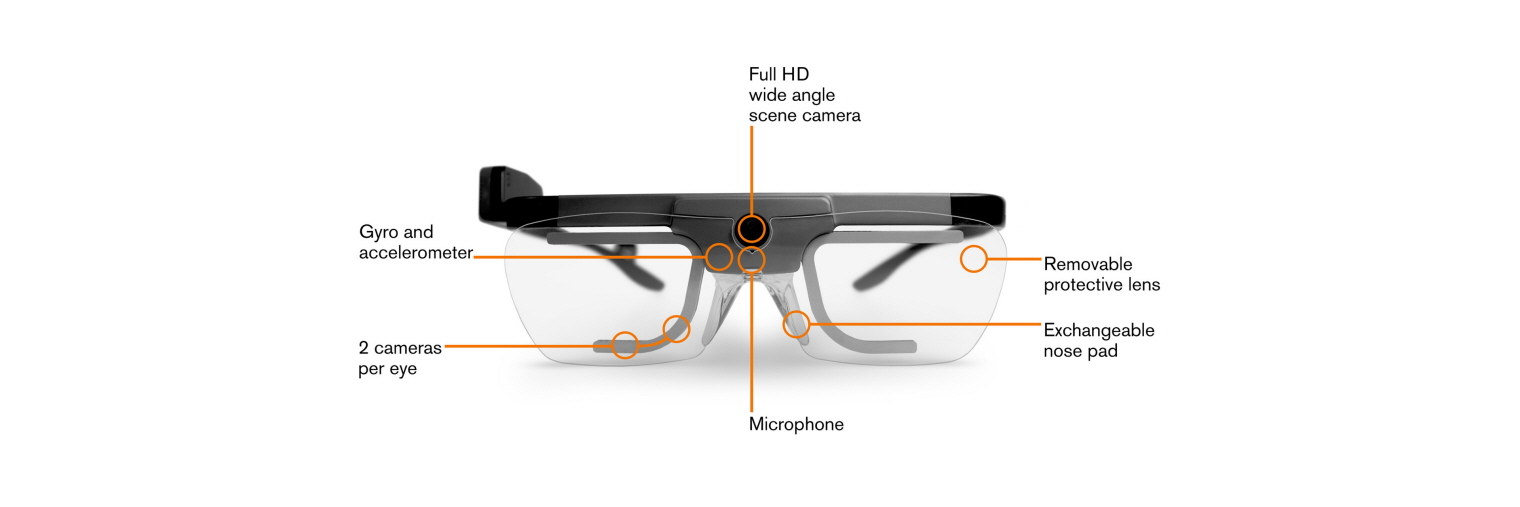
\includegraphics[width=14.07in]{./pictures/tobiiglasses2} 

}

\caption{Tobii Pro Glasses 2; Source: https://www.tobiipro.com/product-listing/tobii-pro-glasses-2/}\label{fig:tobiiglasses2}
\end{figure}

\begin{figure}

{\centering 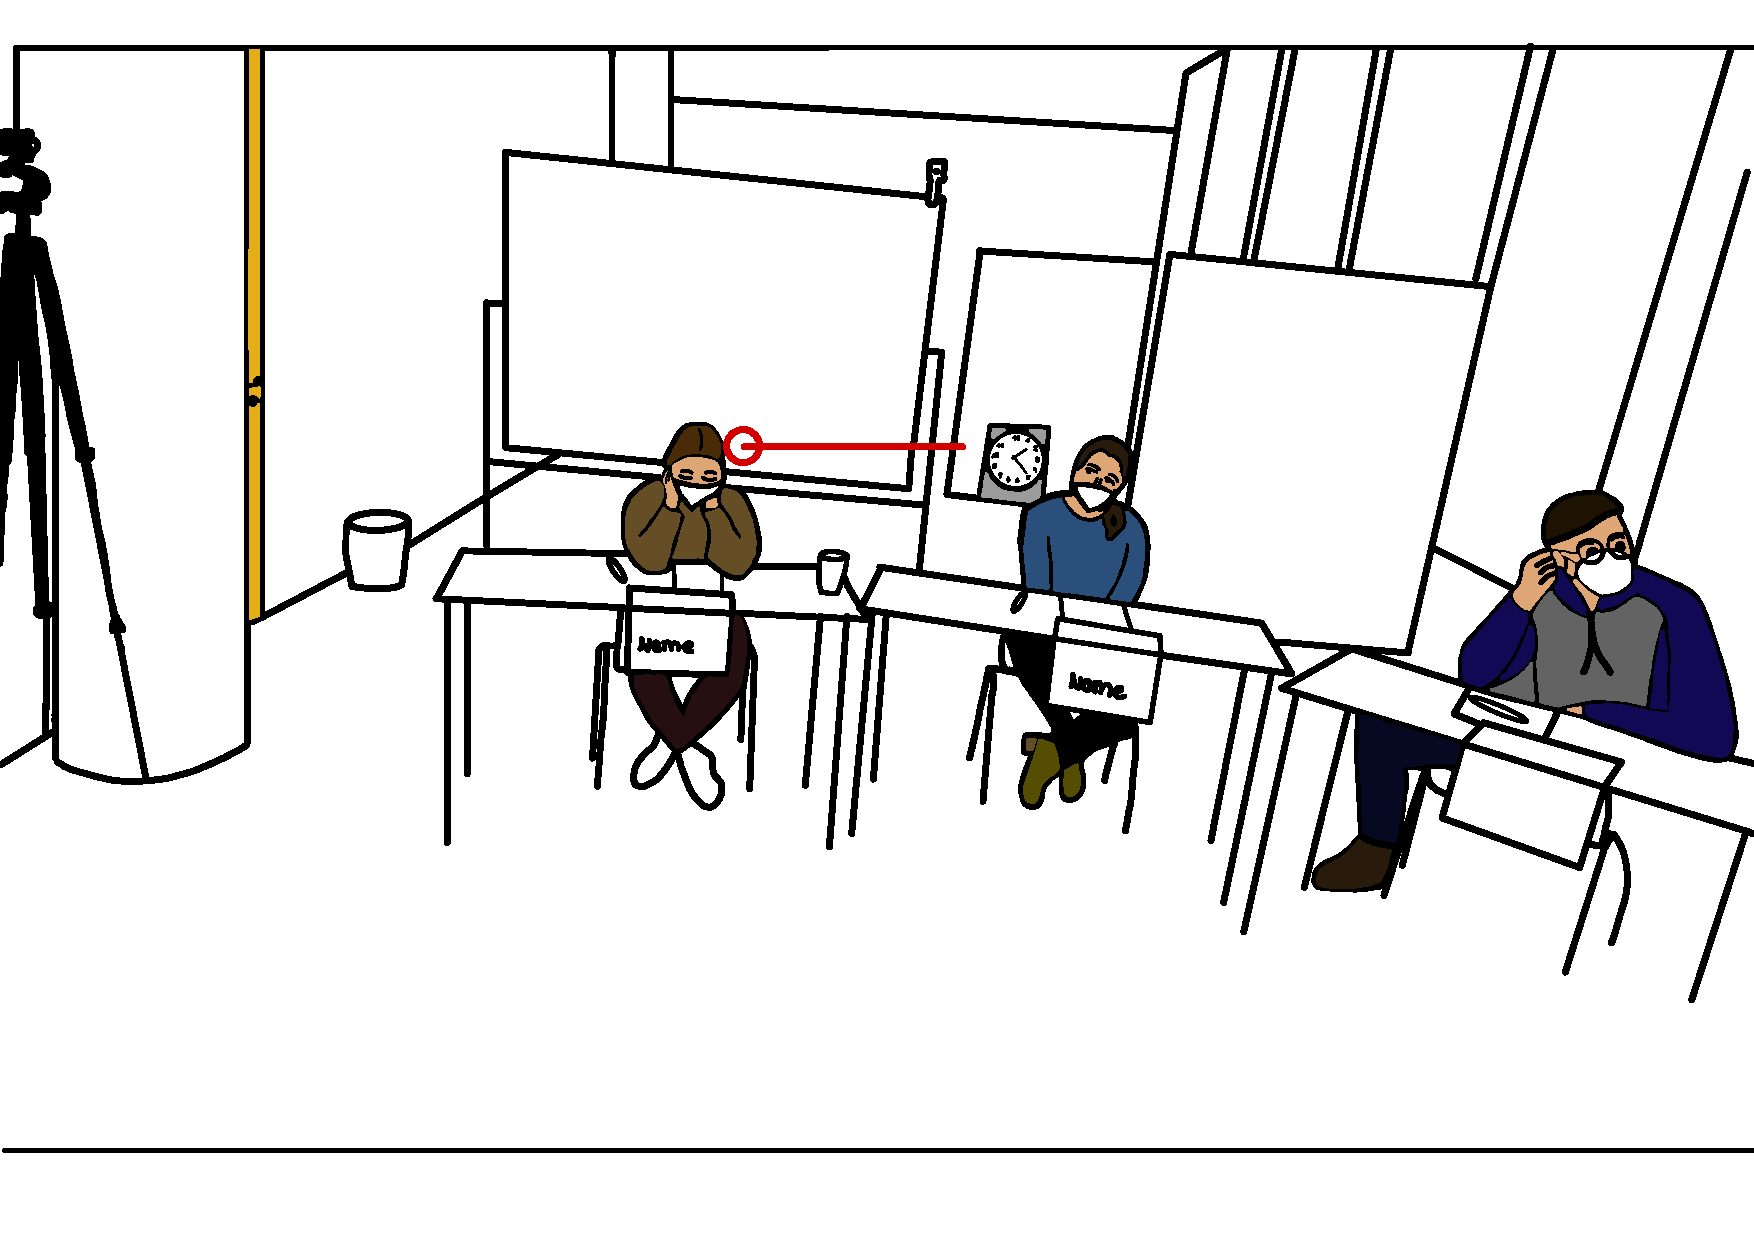
\includegraphics{./pictures/teachersgaze} 

}

\caption{Teacher's Gaze Point}\label{fig:teachersgaze}
\end{figure}

\paragraph{Teachers' visual focus of attention}\label{teachers-visual-focus-of-attention}

Teachers' areas of interest (AOI) were identified as targets where teachers looked during the micro-teaching-unit using Tobii Pro Lab Analyzer Software Version 1.171. In the present study, general AOIs where defined as the student group, the students' nametags, the teacher material, the students' material, the board and non-instructional material in the classroom (wall, window, floor). These AOIs were coded during the manual fixation mapping process during the entire micro-teaching-unit. Additionally, the disruptive person was coded as an event-based AOI only over the duration of the disruption.

--\textgreater{} Only eye-tracking video recordings with 70 \% and above gaze sample percentages were selected for the study to ensure that one or both eyes were detected during 70 \% of the recording's duration (Chaudhuri et al, 2022). Screenshots of the video recordings were used to define the AOI in the eye-tracking videos. The coder started manual gaze mapping when the teacher entered the classroom and ended coding when the micro-teaching-unit ended. The start and end of the micro-teaching-unit was defined by a visual and acoustical signal. The two coders who were assigned to code the eye-tracking videos student employees who studied to be teachers and received a detailed introduction to the software. The intercoder reliability was checked by double coding 20 \% of the videos from the whole dataset. Double coding agreement ranged from XXX \% to XXX \%.

We coded each fixation using the Attention Filter in Pro Lab with the velocity threshold parameter set to 100 degrees/second instead of the default 30 degrees/second. This filter is suitable for dynamic situations to study attention without separating any eye movements. By choosing the Attention Filter typical fixations, most VOR (Vestibulo-ocular reflex), smooth pursuit eye movements, and slow saccades are classified as fixations.

The relevant fixation metrics such as number of fixations, the total duration of fixations and time to first fixation on the relevant event (disruptive person) were obtained by exporting an interval-based TSV file from the Tobii Pro Lab Analyzer Software. The total fixation duration and the time to first fixation metrics were measured in milliseconds (ms) and the number of fixation in counts as an integer. To calculate the average fixation of durations for all AOIs, we divided the total duration of fixations by the number of fixations for each AOI.

\subsubsection{Video data}\label{video-data}

\paragraph{Apparatus}\label{apparatus-1}

The speech, sounds and voices of the participants were recorded with Zoom H3-VR Ambient Recorder installed in the middle of the lab setting (see set up plan \ref{fig:setup}. The Zoom H3-VR recorded with four built-in mics arranged in an Ambisonic array with a bitrate of 4608 kBits/s. Movements, facial expressions and gestures of the subjects were recorded with four Go Pro Hero 7 black cameras from different angles (see set up plan \ref{fig:setup}. The videos were recorded with a sampling rate of 50 Hz in a video resolution with 1920 x 1080 at 50 frames per second in 16:9 format with a linear field of view.

\paragraph{Videography: Coding scheme for expertise indicators}\label{videography-coding-scheme-for-expertise-indicators}

Part of the test procedure was that the subject taught a 15min micro-teaching-unit and was disrupted by the students in the class. The participant's behavior and reaction to the disruption were recorded using video cameras and then evaluated with two self developed coding schemes to assess the teacher's reaction on the one hand and the time on task during the unit. Both aspects are important indicators of teaching quality and are therefore used as another measure to make differences in expertise visible and measurable.

Video analysis was chosen as the research method for evaluating the teacher's reaction to classroom disruptions because it offers numerous advantages. In contrast to transcripts or audio-only recordings, a video also shows nonverbal forms of communication, which is emphasized here, as well as the entire complex lesson excerpt in which many things happen simultaneously (cf.~Krammer \& Reusser, 2012, p.~47f). Video data can also be viewed and analyzed over and over again from different perspectives (Petko et al., 2003, p.~265). The possible problem of selectivity (cf.~Petko et al., 2003, p.~271), i.e., the fact that only a section of the events can be shown due to the position and perspective of the camera, was countered by recording the lessons from a total of four cameras. In this way, a case of doubt can be analyzed from several angles. Another challenge can be the so-called `camera effect', i.e.~that the filmed persons feel disturbed and act differently than usual and less naturally. However, Petko et al.~(2003) conclude, despite filming with a camera person at the time, that there is little reason to believe that teachers can easily change their teaching style from one lesson to the next (p.~270) and that it should not be assumed that the mere presence of a camera has significantly improved or worsened teaching' (p.~270). In the `ProVisioNET' survey, four very small cameras were placed in the room and their presence was barely noticeable. Accordingly, it is assumed that no major nuisance emanates from them.

Schnettler and Knoblauch (2009, p.~227) distinguish `natural' and edited video data, depending on whether the situation was created specifically for the recording or whether the situation was influenced as little as possible or not at all. In the survey for this paper, although the subjects were to act exactly as they would have done without a camera, the classroom disruptions were scripted events that were performed by the actors.

\subparagraph{Teachers' Reaction to disruptions}\label{teachers-reaction-to-disruptions}

The evaluation of the teacher's reaction to the disruptions was conducted as a systematic observation using a category system with fixed categories and instructions. This corresponds to a highly inferential procedure, which is combined with an event sampling procedure (cf.~Lotz et al., 2013, p.~359).

A theory-based coding scheme was developed as an observation tool for classroom observation. The coding of the reactions was done in seven levels. Based on the literature on effective approaches to classroom disruptions, nonverbal response was given Code 1 as the best variant because it best accommodates the classroom management strategies of presence and overlapping (Gold \& Holodynski, 2015; cf. Kounin, 2006) by not interrupting the flow of instruction. Code 2 or Code 3 was assigned for a brief verbal expression with or without a preceding nonverbal response. A brief, timely, and purposeful rebuke of the disruptive student is considered by Kounin (2009, p.~99), among others, to be an important component of the strategy of presence and thus demonstrates good classroom management. If the teacher reacts non-verbally and at the same time with a longer verbal statement, code 4 was assigned, because the flow of the lesson was already noticeably delayed. There were two possibilities, if there was no reaction: If the teacher deliberately ignored the disruption, code 5 was assigned. If the teacher did not notice the disruption, code 6 was assigned, because then no effective monitoring was realized (cf. Gold \& Holodynski, 2015).If the reaction to the disruption was dysfunctional, i.e., if the teacher shows an inappropriate reaction, such as explaining the class rules for a very long time in the case of an insignificant disruption, code 7 was assigned. According to Gippert et al.~(2019), there is a relational error in such cases, as the intensity of the student response should be relative to the disruptive behavior (p.~2).

In developing the coding system, questions initially aroused about how descriptions of responses should be made and in what order (especially codes 3-4). Initially, it was planned to assign code 3 for a nonverbal and simultaneously long verbal response and code 4 for a purely verbal response. However, during the initial trial coding of the videos, it became apparent that it was difficult to reliably distinguish nonverbal reactions to a classroom disruption from normal facial expressions and gestures of the teacher when talking. Moreover, during a prolonged verbal utterance, nonverbal signs could virtually always be detected. Furthermore, a category for short, purely verbal reactions was missing.

After developing and reviewing the coding system, the observers coordinated and the consistency of their ratings was verified. For the evaluation, the individual videos of the sample were then coded and the data transferred to an Excel file.

Test quality criteria

In the construction of the video analysis method, attention was paid to compliance with the quality criteria of objectivity, reliability and validity.

In order to ensure implementation objectivity, uniform implementation conditions were created. In the experimental manual of the ProVisioNET study, the survey procedure is described in detail, so that it is the same for each participant. On the one hand, the objectivity of the evaluation was given by the processing in the R. On the other hand, prior to the analysis of the videos, a precise coding scheme, which precisely describes the individual codes, explains them and contains examples, was created and discursively discussed in the team (see chapter 4.4.1). This coding scheme was tested and revised in a piloting process, which increased the internal validity of the method. Interrater reliability was determined for the two raters using sample ratings of the same videos. Percent agreement yielded 77.8\% and a Cohen's Kappa of k = 0.6, which is a satisfactory value according to Landis \& Koch (1977). Interpretive objectivity was ensured by specifying scientific hypotheses that then had to be neutrally tested.

With the help of scripted behavioral instructions for students in the instructional unit, a high degree of standardization was achieved that is not present in the normal school setting. The lessons were recorded with several video cameras from different angles and an audio recorder. This means a big advantage compared to the subjective evaluation of observers in real time. In addition, video recordings can be viewed multiple times, by different people or from different perspectives. Thus, a high measurement accuracy (reliability) is given {[}cf.@mayring2005auswertung{]}. All measures taken contribute to increase the validity of the method. However, it cannot be answered whether the coding scheme is completely valid, because a validation with the help of another measuring instrument was not possible. Therefore, it could not be controlled whether the collected construct is related to other similar constructs.

\subparagraph{Coding Time on Task}\label{coding-time-on-task}

XXX

\subsubsection{Questionnaie data}\label{questionnaie-data}

\paragraph{Presence Questionnaire}\label{presence-questionnaire}

After each micro-teaching-unit, the three actors answered items on teaching quality using a validated questionnaire (Helmke et al., 2014) and self developed scales on the teacher's presence behavior derived from the research literature. In addition, subjects were asked to give a self-assessment on classroom management by completing the same questionnaire after each micro-teaching-unit. The questionnaire was a 4-point Likert scale (1 = Strongly Disagree; 2 = Disagree; 3 = Agree; 4 = Strongly Agree).

Bilanz:
LB01\_01 Bilanz: Die Lernenden haben in dieser Unterrichtslektion etwas dazu gelernt.
LB01\_02 Bilanz: Die Lernenden haben sich in dieser Unterrichtslektion wohl gefühlt.
LB01\_03 Bilanz: Mediennutzung und Sozialformen waren dem Inhalt und der Situation der Unterrichtslektion angemessen.

Klassenmanagement:
LM01\_01 Klassenmanagement: Die gesamte Unterrichtslektion wurde für den Lernstoff verwendet.
LM01\_02 Klassenmanagement: Ich habe alles mitbekommen, was in der Klasse passiert ist.
LM01\_03 Klassenmanagement: Den Lernenden war jederzeit klar, was sie tun sollten.
LM01\_04 Klassenmanagement: Die Lernenden konnten ungestört arbeiten.
LM01\_05 Klassenmanagement: Die Lernenden waren die ganze Unterrichtslektion über aktiv bei der Sache.
LM01\_06 Klassenmanagement: Ich habe vieles mit kurzen Blicken und knappen Gesten geregelt.
LM01\_07 Klassenmanagement: Auf Störungen habe ich angemessen reagiert.
LM01\_08 Klassenmanagement: Bei Störungen gab ich den Lernenden ein klares STOP-Signal.

Redeanteil:
LO01\_01 Redeanteil: Wieviel Prozent der gesamten Unterrichtslektion hat nach Ihrer Schätzung Ihr eigener Redeanteil eingenommen? \ldots{} \%
LO01\_02 Redeanteil: Wenn ich Fragen oder Aufgaben gestellt habe, habe ich den Lernenden folgende Zeit (in Sekunden) zum Nachdenken gegeben \ldots{} Sekunden

Präsenz:
LP01\_01 Präsenzindikatoren: Ich hatte eine aufrechte, der Klasse zugewandte Körperhaltung.
LP01\_02 Präsenzindikatoren: Ich habe den Lernenden direkt in die Augen geschaut.
LP01\_03 Präsenzindikatoren: Ich habe meine Position im Raum bewusst eingesetzt und variiert.
LP01\_04 Präsenzindikatoren: Ich habe alle oft angesehen.
LP01\_05 Präsenzindikatoren: Meine Artikulation, Lautstärke und Tonhöhe waren angemessen.
LP01\_06 Präsenzindikatoren: Meine Sprechgeschwindigkeit und Sprechpausen waren angemessen.
LP01\_07 Präsenzindikatoren: Mein Sprechanteil an der gesamten Sprechzeit der Unterrichtslektion war angemessen.
LP01\_08 Präsenzindikatoren: Meine Gestik und Mimik waren abwechslungsreich und ausdrucksstark.

Natürliches Verhalten:
LV01\_01 Natürliches Verhalten: Während der Unterrichtslektion habe ich mich sehr natürlich verhalten.
LV01\_02 Natürliches Verhalten: Es war für mich kein Problem, vor einer fiktiven Klasse zu unterrichten.
LV01\_03 Natürliches Verhalten: Beim Unterrichten vor einer fiktiven Klasse habe ich mich so verhalten, wie ich es auch in der Schule tun würde.

\begin{verbatim}
    vars  n mean   sd median trimmed  mad min max range  skew kurtosis   se
\end{verbatim}

LB01\_01 1 84 3.33 0.66 3 3.41 1.48 1 4 3 -0.72 0.43 0.07
LB01\_02 2 84 3.11 0.68 3 3.16 0.00 1 4 3 -0.59 0.79 0.07
LB01\_03 3 84 3.37 0.64 3 3.44 1.48 2 4 2 -0.48 -0.72 0.07
LM01\_01 4 84 3.32 0.73 3 3.43 1.48 1 4 3 -0.93 0.67 0.08
LM01\_03 5 84 3.36 0.53 3 3.35 0.00 2 4 2 0.10 -1.02 0.06
LM01\_04 6 84 3.23 0.65 3 3.28 0.00 2 4 2 -0.24 -0.74 0.07
LM01\_05 7 84 2.71 0.69 3 2.68 0.00 1 4 3 -0.02 -0.34 0.07
LM01\_06 8 84 2.54 0.84 2 2.53 1.48 1 4 3 0.19 -0.67 0.09
LM01\_07 9 84 3.27 0.65 3 3.34 0.00 2 4 2 -0.32 -0.76 0.07
LM01\_08 10 84 3.02 0.76 3 3.07 0.00 1 4 3 -0.53 0.06 0.08
LP01\_01 11 84 3.33 0.65 3 3.41 1.48 2 4 2 -0.43 -0.76 0.07
LP01\_02 12 84 3.33 0.63 3 3.40 0.74 2 4 2 -0.38 -0.73 0.07
LP01\_03 13 84 2.89 0.78 3 2.88 1.48 1 4 3 0.03 -1.03 0.08
LP01\_04 14 84 3.52 0.59 4 3.59 0.00 2 4 2 -0.78 -0.41 0.06
LP01\_05 15 84 3.49 0.57 4 3.53 0.00 2 4 2 -0.53 -0.77 0.06
LP01\_06 16 84 3.19 0.70 3 3.24 1.48 2 4 2 -0.27 -0.99 0.08
LP01\_07 17 84 3.00 0.68 3 3.01 0.00 1 4 3 -0.23 -0.16 0.07
LP01\_08 18 84 2.90 0.67 3 2.90 0.00 1 4 3 -0.13 -0.24 0.07
LV01\_01 19 84 3.23 0.68 3 3.29 0.00 1 4 3 -0.53 0.05 0.07
LV01\_02 20 84 3.32 0.84 4 3.44 0.00 1 4 3 -1.01 0.14 0.09
LV01\_03 21 84 3.19 0.75 3 3.25 1.48 1 4 3 -0.49 -0.58 0.08
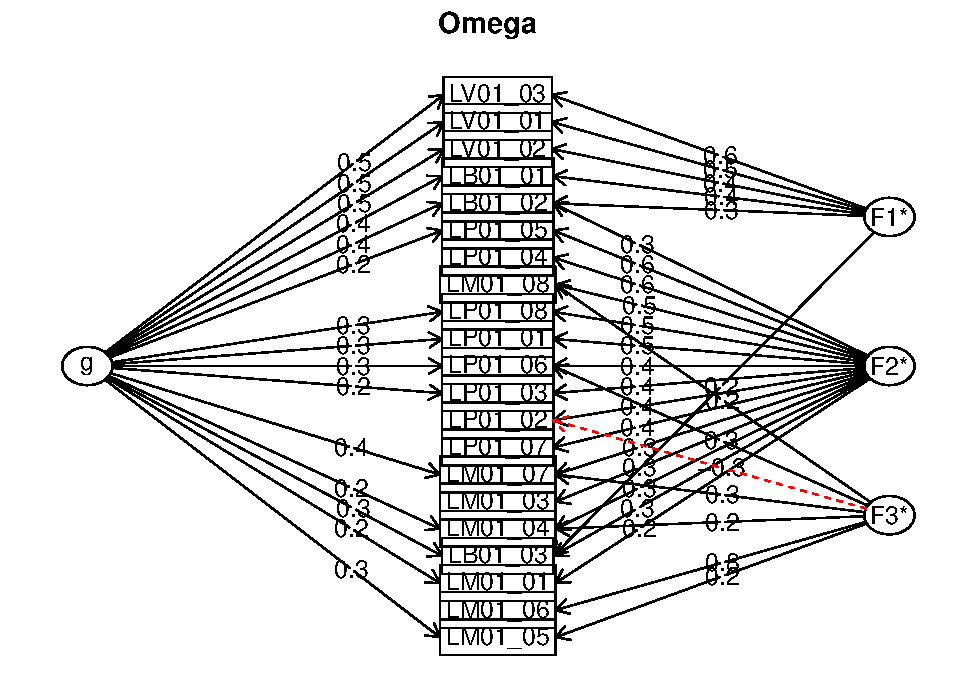
\includegraphics{paper_methods_files/figure-latex/presence_questionnaire-1.pdf} Omega
Call: omegah(m = m, nfactors = nfactors, fm = fm, key = key, flip = flip,
digits = digits, title = title, sl = sl, labels = labels,
plot = plot, n.obs = n.obs, rotate = rotate, Phi = Phi, option = option,
covar = covar)
Alpha: 0.83
G.6: 0.88
Omega Hierarchical: 0.34
Omega H asymptotic: 0.4
Omega Total 0.86

Schmid Leiman Factor loadings greater than 0.2
g F1* F2* F3* h2 h2 u2 p2 com
LB01\_01 0.41 0.38 0.34 0.34 0.66 0.49 2.35
LB01\_02 0.43 0.33 0.29 0.38 0.38 0.62 0.49 2.70
LB01\_03 0.34 0.23 0.27 0.25 0.25 0.75 0.48 2.74
LM01\_01 0.21 0.25 0.13 0.87 0.32 2.88
LM01\_03 0.32 0.12 0.88 0.08 1.33
LM01\_04 0.20 0.29 0.24 0.18 0.82 0.23 2.81
LM01\_05 0.29 0.24 0.20 0.20 0.80 0.43 3.22
LM01\_06 0.20 0.77 0.63 0.63 0.37 0.06 1.16
LM01\_07 0.42 0.20 0.34 0.31 0.42 0.42 0.58 0.41 3.32
LM01\_08 0.48 0.23 0.32 0.32 0.68 0.06 1.78
LP01\_01 0.27 0.46 0.29 0.29 0.71 0.25 1.70
LP01\_02 0.42 -0.30 0.27 0.27 0.73 0.02 1.85
LP01\_03 0.21 0.43 0.23 0.23 0.77 0.20 1.51
LP01\_04 0.58 0.38 0.38 0.62 0.05 1.23
LP01\_05 0.24 0.63 0.46 0.46 0.54 0.12 1.30
LP01\_06 0.32 0.43 0.34 0.41 0.41 0.59 0.26 2.84
LP01\_07 0.41 0.19 0.81 0.02 1.17
LP01\_08 0.28 0.47 0.35 0.35 0.65 0.22 2.15
LV01\_01 0.53 0.46 0.53 0.53 0.47 0.54 2.19
LV01\_02 0.49 0.44 0.45 0.45 0.55 0.53 2.10
LV01\_03 0.48 0.58 0.60 0.60 0.40 0.38 2.19

With Sums of squares of:
g F1* F2* F3* h2
2.0 1.2 2.8 1.2 2.8

general/max 0.71 max/min = 2.41
mean percent general = 0.27 with sd = 0.18 and cv of 0.68
Explained Common Variance of the general factor = 0.28

The degrees of freedom are 150 and the fit is 2.42
The number of observations was 84 with Chi Square = 176.97 with prob \textless{} 0.065
The root mean square of the residuals is 0.07
The df corrected root mean square of the residuals is 0.08
RMSEA index = 0.045 and the 10 \% confidence intervals are 0 0.072
BIC = -487.65

Compare this with the adequacy of just a general factor and no group factors
The degrees of freedom for just the general factor are 189 and the fit is 4.53
The number of observations was 84 with Chi Square = 337.7 with prob \textless{} 1.7e-10
The root mean square of the residuals is 0.16
The df corrected root mean square of the residuals is 0.17

RMSEA index = 0.096 and the 10 \% confidence intervals are 0.08 0.114
BIC = -499.73

Measures of factor score adequacy\\
g F1* F2* F3*
Correlation of scores with factors 0.69 0.66 0.86 0.83
Multiple R square of scores with factors 0.47 0.44 0.75 0.69
Minimum correlation of factor score estimates -0.06 -0.13 0.49 0.38

Total, General and Subset omega for each subset
g F1* F2* F3*
Omega total for total scores and subscales 0.86 0.78 0.79 0.52
Omega general for total scores and subscales 0.34 0.42 0.17 0.10
Omega group for total scores and subscales 0.40 0.37 0.63 0.42

\begin{table}[h]

\begin{center}
\begin{threeparttable}

\caption{\label{tab:presence_questionnaire}Scale analysis for teachers' self-assessment}

\tiny{

\begin{tabular}{lllllllll}
\toprule
 & \multicolumn{1}{c}{N Items} & \multicolumn{1}{c}{M} & \multicolumn{1}{c}{SD} & \multicolumn{1}{c}{Min} & \multicolumn{1}{c}{Max} & \multicolumn{1}{c}{Skewness} & \multicolumn{1}{c}{Kurtosis} & \multicolumn{1}{c}{Alpha}\\
\midrule
Classroom Management & 7.00 & 3.06 & 0.39 & 2.14 & 4.00 & 0.11 & 2.61 & 0.63\\
Balance & 3.00 & 3.27 & 0.52 & 1.67 & 4.00 & -0.49 & 3.14 & 0.69\\
Presence & 8.00 & 3.21 & 0.40 & 2.12 & 3.88 & -0.38 & 2.44 & 0.74\\
Natural Behavior & 3.00 & 3.25 & 0.63 & 1.33 & 4.00 & -0.72 & 3.14 & 0.78\\
\bottomrule
\end{tabular}

}

\end{threeparttable}
\end{center}

\end{table}

\paragraph{Teachers' perception of disruption and confidence using Rating scales}\label{teachers-perception-of-disruption-and-confidence-using-rating-scales}

Two self-developed 11-point rating scales were used to record how disruptive the individual disruptions were perceived by the subjects and how confident they felt in dealing with the disruptions. Data for rating scales were collected during the Stimulted Recall Interview, where the experimenter watched the pre-recorded eye-tracking video with the subject.

The questionnaire included nine questions for each scripted disruptive event. The subjects did not have to complete the questionnaire themselves at any time, as this was done by the experimenter.

For the present study, the following two questions from the interview were relevant:
1. ``How disruptive was this event for you?''
2. ``How confident did you feel in dealing with this event?''

Both questions were answered using a scale ranging from 0 to 10. On this scale, 0 stood for ``not at all disruptive'' or ``not at all safe'' and 10 for ``extremely disturbing'' or ``extremely safe.''

With these rating scales, the subjects indicated their personal subjective feeling towards the individual lesson disruption. Rating scales usually consist of a number of clearly arranged categories that can be presented visually in a variety of ways (Albers, Klapper, Konradt, Walter, \& Wolf, 2009, p. 67f). In the present questionnaire, the numerical representation with eleven answer options (0-10) was used. There was no specific designated neutral position. In this questionnaire, the middle category 5 was not interpreted as a neutral position. In order to avoid misinterpretations of the scaling, the questionnaire was described verbally by the experimenter and follow-up questions from the test subjects were possible at any time. With regard to the quality criteria, it should be made clear that complete objectivity in answering the two questions is given by the rating scales. The question remained the same for all subjects and no additional comments were made. Validity can also be assumed for the questionnaire, since the subjects couls ask follow-up questions and thus uncertainties were clarified. However, similar to the video data, there was no perfect reliability with this survey instrument, because in a few exceptional cases, for example, the experimenter forgot to ask the subject the relevant questions.

\paragraph{Situational Jugdement Test of Strategic Knowledge of Classroom Management}\label{situational-jugdement-test-of-strategic-knowledge-of-classroom-management}

To assess the strategic knowledge of classroom management, subjects answered a Situational Judgement Test (SJT, (Gold \& Holodynski, 2015)). In the questionnaire, participants were given hypothetical school scenarios with five to six response strategies for which they had to evaluate the effectiveness of each strategy on a 6-point rating scale from 1 (A) to 6 (F) according to school grades (see example scenario XXX REFERENZ EINFÜGEN). Depending on the grade given to each strategy, scores were converted in an SPSS syntax resulting in scores ranging from 0 to 1 for each participant.

In developing the test procedure, the authors divided the concept of classroom management into three main aspects: \emph{Monitoring}, \emph{managing momentum} (structuring) and \emph{rules and routines} (Gold \& Holodynski, 2015, p. 230f).

\emph{Monitoring} includes proactive strategies such as omnipresence. This means, the teacher is always informed about the students' behavior, regulates it and reports it back to them. The second strategy is overlapping. In this case, the teacher is able to control several teaching processes at the same time. Monitoring means also reactive strategies of supervision, which also includes the effective handling of classroom disruptions {[}cf.~ibid.; Kounin (2006), p.~89ff{]}. --\textgreater{}

By \emph{managing momentum} (structuring), Gold and Holodynski (2015) understand the skillful control of teaching processes so that they can run smoothly and without delays, taking into account the students' level of understanding and attention (Kounin, 2006, p. 101ff). They also include the group focus specifically identified by Kounin (Kounin, 2006, p. 117ff), i.e.~mobilizing the whole class and demanding accountability (Gold \& Holodynski, 2015, p. 231).

The third facet of classroom management, establishing \emph{rules, routines and rituals}, supports the other two facets and offers pupils orientation and structure in everyday school life (cf.~ibid.).

The construction of the SJT included 14 scenarios that were based on transcribed classroom videos from Germany. For the 14 scenarios, response strategies were derived from evidence-based and theoretical principles by 17 experts on classroom management. With the exception of scenario 5, which was subsequently excluded, the 17 experts agreed on an appropriate level of content validity for all other scenarios (cf.~ibid.). For the validation of the strategies, pair comparisons were made between different strategies and the frequencies were calculated in relation to the expert responses (cf.~ibid., p.~238). Scenarios 10 and 12 were excluded from further analysis because they did not reach the minimum level of agreement (cf.~ibid.).

The construct validity of the SJT with the other 11 scenarios and the sensitivity to differences in strategic knowledge was then examined in a pilot study with 98 trainee teachers and their results validated in a cross-validation with a larger sample (cf.~ibid., p.~238ff). Despite limitations in reliability, the test was confirmed to have content and construct validity (cf.~ibid., p.~243). On the basis of these results, sufficient reliability and validity of the SJT test procedure was assumed.

The scenarios could each be assigned to one facet of the mentioned classroom management: Scenarios 1-4 cover the facet \emph{monitoring}, scenarios 6-9 the facet \emph{managing momentum} and scenarios 11-14 the facet \emph{rules and routines}.

In the current study, objectivity of application was ensured by the questionnaire-format, the written instructions and by a detailed test administration manual of the study \emph{ProVisioNET}. The objectivity of analysis was given by processing the obtained questionnaire data in R (Version 4.3.3; R Core Team, 2021) and the R-packages \emph{apaTables} (Version 2.0.8; Stanley, 2021), \emph{ARTofR} (Version 0.4.1; Zhang, 2021), \emph{cowplot} (Version 1.1.3; Wilke, 2020), \emph{DescTools} (Version 0.99.54; Andri et mult. al., 2022), \emph{dplyr} (Version 1.1.4; Wickham, François, Henry, \& Müller, 2022), \emph{forcats} (Version 1.0.0; Wickham, 2021), \emph{formattable} (Version 0.2.1; Ren \& Russell, 2021), \emph{ggmosaic} (Jeppson, Hofmann, \& Cook, 2021), \emph{ggplot2} (Version 3.5.1; Wickham, 2016), \emph{ggrepel} (Version 0.9.5; Slowikowski, 2021), \emph{ggthemes} (Version 5.1.0; Arnold, 2021), \emph{gridExtra} (Version 2.3; Auguie, 2017), \emph{haven} (Version 2.5.4; Wickham \& Miller, 2021), \emph{imputeTS} (Version 3.3; Moritz \& Bartz-Beielstein, 2017), \emph{janitor} (Version 2.2.0; Firke, 2021), \emph{kableExtra} (Version 1.4.0; Zhu, 2021), \emph{knitr} (Version 1.47; Xie, 2015), \emph{lme4} (Version 1.1.35.4; Bates, Mächler, Bolker, \& Walker, 2015), \emph{ltm} (Version 1.2.0; Rizopoulos, 2006), \emph{lubridate} (Version 1.9.3; Grolemund \& Wickham, 2011), \emph{MASS} (Version 7.3.60.0.1; Venables \& Ripley, 2002), \emph{Matrix} (Version 1.6.5; Bates \& Maechler, 2021), \emph{moments} (Version 0.14.1; Komsta \& Novomestky, 2015), \emph{msm} (Version 1.7.1; Jackson, 2011), \emph{needs} (Version 0.0.3; Katz, 2016), \emph{papaja} (Version 0.1.2; Aust \& Barth, 2020), \emph{polycor} (Version 0.8.1; Fox, 2022), \emph{psych} (Version 2.4.6.26; William Revelle, 2024), \emph{purrr} (Version 1.0.2; Henry \& Wickham, 2020), \emph{readr} (Version 2.1.5; Wickham, Hester, \& Bryan, 2021), \emph{readxl} (Version 1.4.3; Wickham \& Bryan, 2019), \emph{rgeos} (Bivand \& Rundel, 2021), \emph{rlang} (Version 1.1.4; Henry \& Wickham, 2022), \emph{rnaturalearth} (South, 2017a, 2017b), \emph{rnaturalearthdata} (South, 2017b), \emph{rstatix} (Version 0.7.2; Kassambara, 2023), \emph{sf} (E. Pebesma, 2018), \emph{sjlabelled} (Version 1.2.0; Lüdecke, 2022), \emph{sjPlot} (Version 2.8.16; Lüdecke, 2021), \emph{sp} (E. J. Pebesma \& Bivand, 2005), \emph{stringr} (Version 1.5.1; Wickham, 2019), \emph{tibble} (Version 3.2.1; Müller \& Wickham, 2021), \emph{tidyr} (Version 1.3.1; Wickham \& Girlich, 2022), \emph{tidyverse} (Version 2.0.0; Wickham et al., 2019), \emph{tinylabels} (Version 0.2.4; M. Barth, 2022), \emph{viridis} (Version 0.6.5; Garnier et al., 2021a, 2021b), \emph{viridisLite} (Version 0.4.2; Garnier et al., 2021b), and \emph{xtable} (Version 1.8.4; Dahl, Scott, Roosen, Magnusson, \& Swinton, 2019) and IBM SPSS 28.

Since the test was a questionnaire designed to assess strategic knowledge of classroom management of \emph{primary school teachers}, but the sample of the study included several types of schools, changes were made in 10 out of 12 scenarios by deleting the indicated class grade. Only in two scenarios was the class grade information not deleted, as the action alternatives would otherwise not be appropriate without the information.

\begin{table}[h]

\begin{center}
\begin{threeparttable}

\caption{\label{tab:sjt}Scale analysis SJT novices}

\tiny{

\begin{tabular}{lllllllll}
\toprule
 & \multicolumn{1}{c}{N Items} & \multicolumn{1}{c}{M} & \multicolumn{1}{c}{SD} & \multicolumn{1}{c}{Min} & \multicolumn{1}{c}{Max} & \multicolumn{1}{c}{Skewness} & \multicolumn{1}{c}{Kurtosis} & \multicolumn{1}{c}{alpha}\\
\midrule
Monitoring & 4.00 & 0.68 & 0.13 & 0.17 & 0.96 & -1.15 & 6.34 & 0.53\\
Managing Momentum & 5.00 & 0.72 & 0.13 & 0.22 & 0.94 & -1.55 & 6.75 & 0.53\\
Rules and routines & 3.00 & 0.71 & 0.15 & 0.02 & 0.90 & -2.46 & 12.55 & 0.46\\
\bottomrule
\end{tabular}

}

\end{threeparttable}
\end{center}

\end{table}

\begin{table}[h]

\begin{center}
\begin{threeparttable}

\caption{\label{tab:sjt}Scale analysis SJT novices}

\tiny{

\begin{tabular}{lllllllll}
\toprule
 & \multicolumn{1}{c}{N Items} & \multicolumn{1}{c}{M} & \multicolumn{1}{c}{SD} & \multicolumn{1}{c}{Min} & \multicolumn{1}{c}{Max} & \multicolumn{1}{c}{Skewness} & \multicolumn{1}{c}{Kurtosis} & \multicolumn{1}{c}{alpha}\\
\midrule
Monitoring & 4.00 & 0.71 & 0.11 & 0.51 & 0.93 & 0.07 & 2.49 & 0.40\\
Managing Momentum & 5.00 & 0.72 & 0.12 & 0.51 & 0.95 & -0.02 & 1.86 & 0.41\\
Rules and routines & 3.00 & 0.72 & 0.11 & 0.47 & 0.92 & -0.15 & 2.39 & 0.25\\
\bottomrule
\end{tabular}

}

\end{threeparttable}
\end{center}

\end{table}

XXX FRANZI

\subsection{Procedure}\label{procedure}

The project was conducted as a laboratory study in a cross-sectional study design to investigate whether and how teachers' experience has an influence on the perception of and reaction to classroom disruptions.

In June 2021, the study was piloted with student teachers volunteers to refine the study procedure. Data collection was conducted between July 2021 and Septemper 2022.

Before the data collection, each subject received a personal digital meeting with the experimenter to go over the study procedure and to arrange a date for the data collection. During the digital meeting, the subjects were asked to prepare a 15-minute lesson in a subject and grade of their choice for the data collection.

On the day of a data collection, the first step was to set up the study room at the University of Leipzig. For this, all the appropriate technical equipment was charged and installed in the room (see set up plan {[}REFERENZ EINFÜGEN{]}). Next, all four cameras and the audio recorder were synced via Timecode System.

After the subject arrived, a smart watch was put on to measure the heart rate during the session and to get a pretest time at least 15min before the session started. In addition to the experimenter and the subject, three student assistants from the working group always took part in the data collection, as they represented the class.

After the welcome, the subject was again briefed about the study. It was explicitly pointed out that the student assistants would act as the class and simulate typical class events during the lesson. The subject was asked in advance to behave as naturally as possible during the entire time. Next, the subjects' written informed consent was obtained and contact details were collected in order to inform all persons participating in the study if a covid infection should occur.

After the introduction, the eye-tracking glasses were adjusted for the subject by inserting contact lenses if necessary and changing the nose pad. To start the eye tracking glasses, the Tobii Glasses must be fitted onto the subject's head via an one-point-calibration. In the calibration process the subject was asked to look at a Calibration Card held in-front of the subject for a few seconds. The experimenter started the recording from Tobii Glasses Controller Software running on a computer.

After starting the eye tracking recording, all other technical devices were also switched on: The four cameras and the audio recorder were controlled via iPad using the BLINK Hup app and could be started simultaneously by synchronization. The ZED camera was started manually on another laptop.

Before the 15-minute lesson, there was a short 10-minute warm-up phase. The phase was divided into two parts and served on the one hand to get the subjects used to the eye-tracking glasses and on the other hand to get used to their class. In the first phase of the warm-up, the game ``name juggling'' was played using two balls. In the game, the subject and the three actors threw two balls at each other and, depending on the color of the ball, called either their own name or that of the target person. After the name juggling, the subjects were supposed to start a conversation. For this, the subject thought of a question for each student and was also asked a question of each student. The content could be anything that interested the participants.

After the warm up phase, the experimenter ensured a manual synchronization of the technique by an acoustic signal in which she clapped her hands loudly twice standing in the middle of the room. After this, another nine-point calibration followed outside the study room in a neighboring room. Before the subject left the room for calibration, the time on the smartwatch was noted, as well as the steps recorded until that point. The subject had to stand at a marked point and look at a board three meters away with nine april tags. The subject was asked to read the nine points aloud in order at a normal speaking speed. This procedure was important to validate the one-point calibration on the one hand and on the other hand to give the subject the feeling of a lesson start, because after this calibration the subject came into the study room to start the 15-minute lesson.

For the micro-teaching lesson, student teachers and experienced teachers were asked to prepare an introduction of 15 minutes which they taught in front of the fictitious class consisting of three student assistants. The actors simulated the nine classroom events during the lesson, derived by research literature. The order of the disruptions as well as the students performing them were fully balanced using Latin Square. The disruptions were only visible for the class on a screen.

\begin{table}[h]

\begin{center}
\begin{threeparttable}

\caption{\label{tab:disruption_categories}Categories of Disruptions (Lohmann, 2015)}

\tiny{

\begin{tabular}{lll}
\toprule
Verbal.Disruption & \multicolumn{1}{c}{Agitation} & \multicolumn{1}{c}{Lack.of.eagerness.to.learn}\\
\midrule
chatting with neighbor & drumming hands & putting head on table\\
whispering with neighbor & clicking pen & looking at phone\\
heckling & snipping with fingers & drawing on a sheet of paper\\
\bottomrule
\end{tabular}

}

\end{threeparttable}
\end{center}

\end{table}

During the lesson, a mobile eye-tracker recorded the subject's gaze behavior and audio data of the lesson. All other sounds and voices were recorded by an audio recorder. To record facial expressions, gestures and movements, four mobile cameras were installed to record the classroom from all perspectives (!!!see figures).

After the lesson, the time was again noted from the smartwatch as well as the subject's steps. The nine-point calibration was also performed again in the neighboring room. This time, however, the subject was asked to wait outside the room until he or she was called in, because four letters from A to D were placed in the study room. The subject was asked to stand facing the board at a marked point in the room and, when given an acoustic signal, to turn around and search the letters and read them aloud in order. This served as a control condition for the speed of the subjects' perceptual ability as no expertise is required for searching letters.

After the letter search, the experimenter clapped twice with the hands to record an acoustic signal for the synchronization of all technical devices. Afterwards, all devices were switched off and the subjects as well as the actors were given a short questionnaire, which contained items to collect demographic information as well as items about the previously given lesson on teaching quality using a validated questionnaire (Helmke et al., 2014) and self developed scales on the teacher's presence behavior derived from the research literature. The completion of the questionnaire took approximately 5 minutes.

In the second part of the study, the experimenter conducted a Stimulated Recall Interview (SRI) with the subject(see in Figure \ref{fig:sri}. The interview was recorded by the ambient recorder and additionally with a software called OBS to record the speech and screen. The recorded eye-tracking video was watched and commented on by the subject while thinking aloud. The interview was structured by a guideline based on a fixed sequence of questions, however the subjects were allowed to answer completely open to these questions. The objective was to collect data that would provide insight into the subjects' thoughts and reactions in relation to the scripted classroom disruptions. The eye-tracking video was not completely re-watched, but stopped at the points where disruptions occurred. After the disruption occurred, the subject was asked to describe what had just happened. If the disruption was noticed, the subject was asked how disruptive the event was at that moment on a scale from 0 to 10. In addition, the subject was asked to reason the given number. In a next step, the experimenter re-played the subject's reaction to the disruption and asked to describe and reason the reaction. The experimenter then asked the subject to rate on a scale from 0 to 10 how confident he/she felt in dealing with the disruption and again to reason the number (for a detailed description of the scale question, see Rating Scales).

\begin{figure}

{\centering 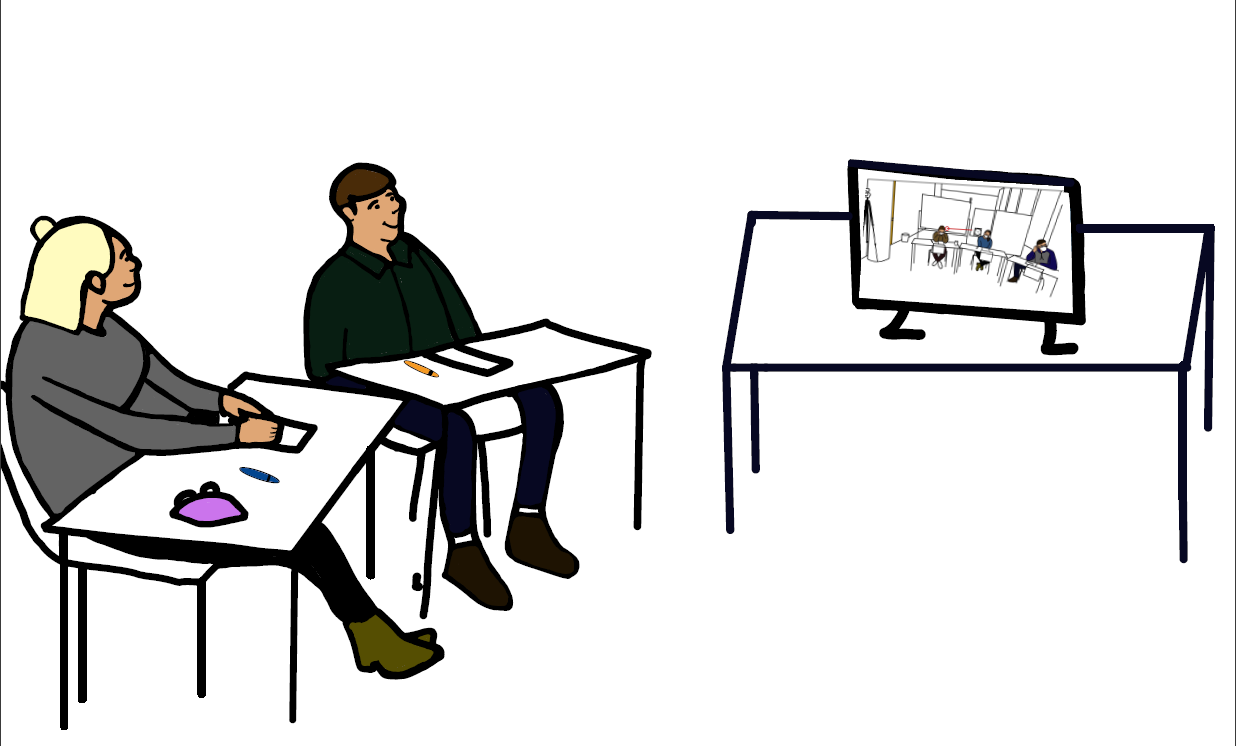
\includegraphics{./pictures/sri} 

}

\caption{Subject and experimenter during the Stimulated Recall Interview}\label{fig:sri}
\end{figure}

Finally, the subjects answered a Situational Judgement Test of Strategic Knowledge of Classroom Management (SJT, Gold \& Holodynski, 2015) in the form of a questionnaire. Here they had to assess teaching scenarios and evaluate their behavior in response to them. The SJT was used to assess strategic knowledge about classroom management. The completion of the entire survey took 15 min on average.

\subsection{Data analysis}\label{data-analysis}

We investigated whether experts and novice teachers differed

All reported data analyses were conducted with the R (Version 4.3.3; R Core Team, 2021) and the R-packages \emph{apaTables} (Version 2.0.8; Stanley, 2021), \emph{ARTofR} (Version 0.4.1; Zhang, 2021), \emph{cowplot} (Version 1.1.3; Wilke, 2020), \emph{DescTools} (Version 0.99.54; Andri et mult. al., 2022), \emph{dplyr} (Version 1.1.4; Wickham et al., 2022), \emph{forcats} (Version 1.0.0; Wickham, 2021), \emph{formattable} (Version 0.2.1; Ren \& Russell, 2021), \emph{ggmosaic} (Jeppson et al., 2021), \emph{ggplot2} (Version 3.5.1; Wickham, 2016), \emph{ggrepel} (Version 0.9.5; Slowikowski, 2021), \emph{ggthemes} (Version 5.1.0; Arnold, 2021), \emph{gridExtra} (Version 2.3; Auguie, 2017), \emph{haven} (Version 2.5.4; Wickham \& Miller, 2021), \emph{imputeTS} (Version 3.3; Moritz \& Bartz-Beielstein, 2017), \emph{janitor} (Version 2.2.0; Firke, 2021), \emph{kableExtra} (Version 1.4.0; Zhu, 2021), \emph{knitr} (Version 1.47; Xie, 2015), \emph{lme4} (Version 1.1.35.4; Bates et al., 2015), \emph{ltm} (Version 1.2.0; Rizopoulos, 2006), \emph{lubridate} (Version 1.9.3; Grolemund \& Wickham, 2011), \emph{MASS} (Version 7.3.60.0.1; Venables \& Ripley, 2002), \emph{Matrix} (Version 1.6.5; Bates \& Maechler, 2021), \emph{moments} (Version 0.14.1; Komsta \& Novomestky, 2015), \emph{msm} (Version 1.7.1; Jackson, 2011), \emph{needs} (Version 0.0.3; Katz, 2016), \emph{papaja} (Version 0.1.2; Aust \& Barth, 2020), \emph{polycor} (Version 0.8.1; Fox, 2022), \emph{psych} (Version 2.4.6.26; William Revelle, 2024), \emph{purrr} (Version 1.0.2; Henry \& Wickham, 2020), \emph{readr} (Version 2.1.5; Wickham et al., 2021), \emph{readxl} (Version 1.4.3; Wickham \& Bryan, 2019), \emph{rgeos} (Bivand \& Rundel, 2021), \emph{rlang} (Version 1.1.4; Henry \& Wickham, 2022), \emph{rnaturalearth} (South, 2017a, 2017b), \emph{rnaturalearthdata} (South, 2017b), \emph{rstatix} (Version 0.7.2; Kassambara, 2023), \emph{sf} (E. Pebesma, 2018), \emph{sjlabelled} (Version 1.2.0; Lüdecke, 2022), \emph{sjPlot} (Version 2.8.16; Lüdecke, 2021), \emph{sp} (E. J. Pebesma \& Bivand, 2005), \emph{stringr} (Version 1.5.1; Wickham, 2019), \emph{tibble} (Version 3.2.1; Müller \& Wickham, 2021), \emph{tidyr} (Version 1.3.1; Wickham \& Girlich, 2022), \emph{tidyverse} (Version 2.0.0; Wickham et al., 2019), \emph{tinylabels} (Version 0.2.4; M. Barth, 2022), \emph{viridis} (Version 0.6.5; Garnier et al., 2021a, 2021b), \emph{viridisLite} (Version 0.4.2; Garnier et al., 2021b), and \emph{xtable} (Version 1.8.4; Dahl et al., 2019) and IBM SPSS 28.

\section{Results}\label{results}

\section{Discussion}\label{discussion}

\newpage

\section{References}\label{references}

\begingroup
\setlength{\parindent}{-0.5in}
\setlength{\leftskip}{0.5in}

\phantomsection\label{refs}
\begin{CSLReferences}{1}{0}
\bibitem[\citeproctext]{ref-albers2009methodik}
Albers, S., Klapper, D., Konradt, U., Walter, A., \& Wolf, J. (2009). \emph{Methodik der empirischen forschung} (Vol. 3). Springer.

\bibitem[\citeproctext]{ref-R-DescTools}
Andri et mult. al., S. (2022). \emph{{DescTools}: Tools for descriptive statistics}. Retrieved from \url{https://cran.r-project.org/package=DescTools}

\bibitem[\citeproctext]{ref-R-ggthemes}
Arnold, J. B. (2021). \emph{Ggthemes: Extra themes, scales and geoms for 'ggplot2'}. Retrieved from \url{https://CRAN.R-project.org/package=ggthemes}

\bibitem[\citeproctext]{ref-R-gridExtra}
Auguie, B. (2017). \emph{gridExtra: Miscellaneous functions for "grid" graphics}. Retrieved from \url{https://CRAN.R-project.org/package=gridExtra}

\bibitem[\citeproctext]{ref-R-papaja}
Aust, F., \& Barth, M. (2020). \emph{{papaja}: {Prepare} reproducible {APA} journal articles with {R Markdown}}. Retrieved from \url{https://github.com/crsh/papaja}

\bibitem[\citeproctext]{ref-R-tinylabels}
Barth, M. (2022). \emph{{tinylabels}: Lightweight variable labels}. Retrieved from \url{https://cran.r-project.org/package=tinylabels}

\bibitem[\citeproctext]{ref-barth2017professionelle}
Barth, V. L. (2017). \emph{Professionelle wahrnehmung von st{ö}rungen im unterricht}. Springer.

\bibitem[\citeproctext]{ref-R-lme4}
Bates, D., Mächler, M., Bolker, B., \& Walker, S. (2015). Fitting linear mixed-effects models using {lme4}. \emph{Journal of Statistical Software}, \emph{67}(1), 1--48. \url{https://doi.org/10.18637/jss.v067.i01}

\bibitem[\citeproctext]{ref-R-Matrix}
Bates, D., \& Maechler, M. (2021). \emph{Matrix: Sparse and dense matrix classes and methods}. Retrieved from \url{https://CRAN.R-project.org/package=Matrix}

\bibitem[\citeproctext]{ref-baumert2006key}
Baumert, J., \& Kunter, M. (2006). Key word: Professional competence of teachers. \emph{ZEITSCHRIFT FUR ERZIEHUNGSWISSENSCHAFT}, \emph{9}(4), 469--520.

\bibitem[\citeproctext]{ref-berliner1994expertise}
Berliner, D. C. (1994). Expertise: The wonders of exemplary performance. \emph{Creating Powerful Thinking in Teachers and Students}, 161--186.

\bibitem[\citeproctext]{ref-R-rgeos}
Bivand, R., \& Rundel, C. (2021). \emph{Rgeos: Interface to geometry engine - open source ('GEOS')}. Retrieved from \url{https://CRAN.R-project.org/package=rgeos}

\bibitem[\citeproctext]{ref-blake2013eye}
Blake, C. (2013). Eye-tracking: Grundlagen und anwendungsfelder. In \emph{Handbuch standardisierte erhebungsverfahren in der kommunikationswissenschaft} (pp. 367--387). Springer.

\bibitem[\citeproctext]{ref-R-xtable}
Dahl, D. B., Scott, D., Roosen, C., Magnusson, A., \& Swinton, J. (2019). \emph{Xtable: Export tables to LaTeX or HTML}. Retrieved from \url{https://CRAN.R-project.org/package=xtable}

\bibitem[\citeproctext]{ref-eckstein2016unterrichtliche}
Eckstein, B., Grob, U., \& Reusser, K. (2016). Unterrichtliche devianz und subjektives st{ö}rungsempfinden. Entwicklung eines instrumentariums zur erfassung von unterrichtsst{ö}rungen. \emph{Empirische P{ä}dagogik (EP)}, \emph{30}(1), 113--129.

\bibitem[\citeproctext]{ref-emmer1982improving}
Emmer, E., Sanford, J., Clements, B., \& Martin, J. (1982). Improving classroom management and organization in junior high schools. \emph{An. Experimental, Investigation. Washington, DC: National Institute}.

\bibitem[\citeproctext]{ref-epstein2002defining}
Epstein, R. M., \& Hundert, E. M. (2002). Defining and assessing professional competence. \emph{Jama}, \emph{287}(2), 226--235.

\bibitem[\citeproctext]{ref-evertson2006classroom}
Evertson, C. M., Weinstein, C. S., et al. (2006). Classroom management as a field of inquiry. \emph{Handbook of Classroom Management: Research, Practice, and Contemporary Issues}, \emph{3}(1), 16.

\bibitem[\citeproctext]{ref-R-janitor}
Firke, S. (2021). \emph{Janitor: Simple tools for examining and cleaning dirty data}. Retrieved from \url{https://CRAN.R-project.org/package=janitor}

\bibitem[\citeproctext]{ref-R-polycor}
Fox, J. (2022). \emph{Polycor: Polychoric and polyserial correlations}. Retrieved from \url{https://CRAN.R-project.org/package=polycor}

\bibitem[\citeproctext]{ref-R-viridis}
Garnier, Simon, Ross, Noam, Rudis, Robert, \ldots{} Cédric. (2021a). \emph{{viridis} - colorblind-friendly color maps for r}. \url{https://doi.org/10.5281/zenodo.4679424}

\bibitem[\citeproctext]{ref-R-viridisLite}
Garnier, Simon, Ross, Noam, Rudis, Robert, \ldots{} Cédric. (2021b). \emph{{viridis} - colorblind-friendly color maps for r}. \url{https://doi.org/10.5281/zenodo.4679424}

\bibitem[\citeproctext]{ref-gegenfurtner2018mobiles}
Gegenfurtner, A., Eichinger, A., Latzel, R., Dietrich, M. P., Barkowsky, M., Glufke, A., \ldots{} Stern, W. (2018). \emph{Mobiles eye-tracking in den angewandten wissenschaften}.

\bibitem[\citeproctext]{ref-gold2015development}
Gold, B., \& Holodynski, M. (2015). Development and construct validation of a situational judgment test of strategic knowledge of classroom management in elementary schools. \emph{Educational Assessment}, \emph{20}(3), 226--248.

\bibitem[\citeproctext]{ref-gold2017using}
Gold, B., \& Holodynski, M. (2017). Using digital video to measure the professional vision of elementary classroom management: Test validation and methodological challenges. \emph{Computers \& Education}, \emph{107}, 13--30.

\bibitem[\citeproctext]{ref-R-lubridate}
Grolemund, G., \& Wickham, H. (2011). Dates and times made easy with {lubridate}. \emph{Journal of Statistical Software}, \emph{40}(3), 1--25. Retrieved from \url{https://www.jstatsoft.org/v40/i03/}

\bibitem[\citeproctext]{ref-grub2020process}
Grub, A.-S., Biermann, A., \& Brünken, R. (2020). Process-based measurement of professional vision of (prospective) teachers in the field of classroom management. A systematic review. \emph{Journal for Educational Research Online}, \emph{12}(3), 75--102.

\bibitem[\citeproctext]{ref-helmke2014unterrichtsdiagnostik}
Helmke, A., Helmke, T., Lenske, G., Pham, G., Praetorius, A.-K., Schrader, F.-W., \& AdeThurow, M. (2014). Unterrichtsdiagnostik mit EMU. \emph{Aus-Und Fortbildung Der Lehrkr{ä}fte in Hinblick Auf Verbesserung Der Diagnosef{ä}higkeit, Umgang Mit Heterogenit{ä}t Und Individuelle F{ö}rderung}, 149--163.

\bibitem[\citeproctext]{ref-R-purrr}
Henry, L., \& Wickham, H. (2020). \emph{Purrr: Functional programming tools}. Retrieved from \url{https://CRAN.R-project.org/package=purrr}

\bibitem[\citeproctext]{ref-R-rlang}
Henry, L., \& Wickham, H. (2022). \emph{Rlang: Functions for base types and core r and 'tidyverse' features}. Retrieved from \url{https://CRAN.R-project.org/package=rlang}

\bibitem[\citeproctext]{ref-R-msm}
Jackson, C. H. (2011). Multi-state models for panel data: The {msm} package for {R}. \emph{Journal of Statistical Software}, \emph{38}(8), 1--29. Retrieved from \url{https://www.jstatsoft.org/v38/i08/}

\bibitem[\citeproctext]{ref-jahn2014professionelle}
Jahn, G., Stürmer, K., Seidel, T., \& Prenzel, M. (2014). Professionelle unterrichtswahrnehmung von lehramtsstudierenden: Eine scaling-up studie des observe-projekts. \emph{Zeitschrift f{ü}r Entwicklungspsychologie Und p{ä}dagogische Psychologie}, \emph{46}(4), 171--180.

\bibitem[\citeproctext]{ref-R-ggmosaic}
Jeppson, H., Hofmann, H., \& Cook, D. (2021). \emph{Ggmosaic: Mosaic plots in the 'ggplot2' framework}. Retrieved from \url{https://CRAN.R-project.org/package=ggmosaic}

\bibitem[\citeproctext]{ref-R-rstatix}
Kassambara, A. (2023). \emph{Rstatix: Pipe-friendly framework for basic statistical tests}. Retrieved from \url{https://CRAN.R-project.org/package=rstatix}

\bibitem[\citeproctext]{ref-R-needs}
Katz, J. (2016). \emph{Needs: Attaches and installs packages}. Retrieved from \url{https://CRAN.R-project.org/package=needs}

\bibitem[\citeproctext]{ref-kleinknecht2013teachers}
Kleinknecht, M., \& Schneider, J. (2013). What do teachers think and feel when analyzing videos of themselves and other teachers teaching? \emph{Teaching and Teacher Education}, \emph{33}, 13--23.

\bibitem[\citeproctext]{ref-klieme2008concept}
Klieme, E., Hartig, J., \& Rauch, D. (2008). The concept of competence in educational contexts. \emph{Assessment of Competencies in Educational Contexts}, \emph{3}, 22.

\bibitem[\citeproctext]{ref-R-moments}
Komsta, L., \& Novomestky, F. (2015). \emph{Moments: Moments, cumulants, skewness, kurtosis and related tests}. Retrieved from \url{https://CRAN.R-project.org/package=moments}

\bibitem[\citeproctext]{ref-kounin2006techniken}
Kounin, J. S. (2006). \emph{Techniken der klassenf{ü}hrung}. Waxmann Verlag.

\bibitem[\citeproctext]{ref-lachner2016makes}
Lachner, A., Jarodzka, H., \& Nückles, M. (2016). What makes an expert teacher? Investigating teachers' professional vision and discourse abilities. \emph{Instructional Science}, \emph{44}(3), 197--203.

\bibitem[\citeproctext]{ref-leinhardt1986cognitive}
Leinhardt, G., \& Greeno, J. G. (1986). The cognitive skill of teaching. \emph{Journal of Educational Psychology}, \emph{78}(2), 75.

\bibitem[\citeproctext]{ref-R-sjPlot}
Lüdecke, D. (2021). \emph{sjPlot: Data visualization for statistics in social science}. Retrieved from \url{https://CRAN.R-project.org/package=sjPlot}

\bibitem[\citeproctext]{ref-R-sjlabelled}
Lüdecke, D. (2022). \emph{Sjlabelled: Labelled data utility functions (version 1.2.0)}. \url{https://doi.org/10.5281/zenodo.1249215}

\bibitem[\citeproctext]{ref-marzano2003classroom}
Marzano, R. J., Marzano, J. S., \& Pickering, D. (2003). \emph{Classroom management that works: Research-based strategies for every teacher}. ASCD.

\bibitem[\citeproctext]{ref-R-imputeTS}
Moritz, S., \& Bartz-Beielstein, T. (2017). {imputeTS: Time Series Missing Value Imputation in R}. \emph{{The R Journal}}, \emph{9}(1), 207--218. \url{https://doi.org/10.32614/RJ-2017-009}

\bibitem[\citeproctext]{ref-R-tibble}
Müller, K., \& Wickham, H. (2021). \emph{Tibble: Simple data frames}. Retrieved from \url{https://CRAN.R-project.org/package=tibble}

\bibitem[\citeproctext]{ref-oser2006competence}
Oser, F. K., Achtenhagen, F., \& Renold, U. (2006). Competence-oriented teacher training: Old research demands and new pathways. In \emph{Competence oriented teacher training} (pp. 1--7). Brill.

\bibitem[\citeproctext]{ref-palmer2005identifying}
Palmer, D. J., Stough, L. M., Burdenski, T. K., Jr, \& Gonzales, M. (2005). Identifying teacher expertise: An examination of researchers' decision making. \emph{Educational Psychologist}, \emph{40}(1), 13--25.

\bibitem[\citeproctext]{ref-R-sf}
Pebesma, E. (2018). {Simple Features for R: Standardized Support for Spatial Vector Data}. \emph{{The R Journal}}, \emph{10}(1), 439--446. \url{https://doi.org/10.32614/RJ-2018-009}

\bibitem[\citeproctext]{ref-R-sp}
Pebesma, E. J., \& Bivand, R. S. (2005). Classes and methods for spatial data in {R}. \emph{R News}, \emph{5}(2), 9--13. Retrieved from \url{https://CRAN.R-project.org/doc/Rnews/}

\bibitem[\citeproctext]{ref-R-base}
R Core Team. (2021). \emph{R: A language and environment for statistical computing}. Vienna, Austria: R Foundation for Statistical Computing. Retrieved from \url{https://www.R-project.org/}

\bibitem[\citeproctext]{ref-R-formattable}
Ren, K., \& Russell, K. (2021). \emph{Formattable: Create 'formattable' data structures}. Retrieved from \url{https://CRAN.R-project.org/package=formattable}

\bibitem[\citeproctext]{ref-R-ltm}
Rizopoulos, D. (2006). Ltm: An r package for latent variable modelling and item response theory analyses. \emph{Journal of Statistical Software}, \emph{17}(5), 1--25. Retrieved from \url{https://doi.org/10.18637/jss.v017.i05}

\bibitem[\citeproctext]{ref-sabers1991differences}
Sabers, D. S., Cushing, K. S., \& Berliner, D. C. (1991). Differences among teachers in a task characterized by simultaneity, multidimensional, and immediacy. \emph{American Educational Research Journal}, \emph{28}(1), 63--88.

\bibitem[\citeproctext]{ref-seidel2014modeling}
Seidel, T., \& Stürmer, K. (2014). Modeling and measuring the structure of professional vision in preservice teachers. \emph{American Educational Research Journal}, \emph{51}(4), 739--771.

\bibitem[\citeproctext]{ref-sherin2007development}
Sherin, M. (2007). \emph{The development of teachers' professional vision in video clubs. Video research in the learning sciences. R. Goldman, r. Pea, b. Barron and SJ derry}. Mahwah, NJ, Lawrence Erlbaum.

\bibitem[\citeproctext]{ref-R-ggrepel}
Slowikowski, K. (2021). \emph{Ggrepel: Automatically position non-overlapping text labels with 'ggplot2'}. Retrieved from \url{https://CRAN.R-project.org/package=ggrepel}

\bibitem[\citeproctext]{ref-R-rnaturalearth}
South, A. (2017a). \emph{Rnaturalearth: World map data from natural earth}. Retrieved from \url{https://CRAN.R-project.org/package=rnaturalearth}

\bibitem[\citeproctext]{ref-R-rnaturalearthdata}
South, A. (2017b). \emph{Rnaturalearthdata: World vector map data from natural earth used in 'rnaturalearth'}. Retrieved from \url{https://CRAN.R-project.org/package=rnaturalearthdata}

\bibitem[\citeproctext]{ref-R-apaTables}
Stanley, D. (2021). \emph{apaTables: Create american psychological association (APA) style tables}. Retrieved from \url{https://CRAN.R-project.org/package=apaTables}

\bibitem[\citeproctext]{ref-treisch2018entwicklung}
Treisch, F. (2018). \emph{Die entwicklung der professionellen unterrichtswahrnehmung im lehr-lern-labor seminar}. Bayerische Julius-Maximilians-Universitaet Wuerzburg (Germany).

\bibitem[\citeproctext]{ref-R-MASS}
Venables, W. N., \& Ripley, B. D. (2002). \emph{Modern applied statistics with s} (Fourth). New York: Springer. Retrieved from \url{https://www.stats.ox.ac.uk/pub/MASS4/}

\bibitem[\citeproctext]{ref-R-ggplot2}
Wickham, H. (2016). \emph{ggplot2: Elegant graphics for data analysis}. Springer-Verlag New York. Retrieved from \url{https://ggplot2.tidyverse.org}

\bibitem[\citeproctext]{ref-R-stringr}
Wickham, H. (2019). \emph{Stringr: Simple, consistent wrappers for common string operations}. Retrieved from \url{https://CRAN.R-project.org/package=stringr}

\bibitem[\citeproctext]{ref-R-forcats}
Wickham, H. (2021). \emph{Forcats: Tools for working with categorical variables (factors)}. Retrieved from \url{https://CRAN.R-project.org/package=forcats}

\bibitem[\citeproctext]{ref-R-tidyverse}
Wickham, H., Averick, M., Bryan, J., Chang, W., McGowan, L. D., François, R., \ldots{} Yutani, H. (2019). Welcome to the {tidyverse}. \emph{Journal of Open Source Software}, \emph{4}(43), 1686. \url{https://doi.org/10.21105/joss.01686}

\bibitem[\citeproctext]{ref-R-readxl}
Wickham, H., \& Bryan, J. (2019). \emph{Readxl: Read excel files}. Retrieved from \url{https://CRAN.R-project.org/package=readxl}

\bibitem[\citeproctext]{ref-R-dplyr}
Wickham, H., François, R., Henry, L., \& Müller, K. (2022). \emph{Dplyr: A grammar of data manipulation}. Retrieved from \url{https://CRAN.R-project.org/package=dplyr}

\bibitem[\citeproctext]{ref-R-tidyr}
Wickham, H., \& Girlich, M. (2022). \emph{Tidyr: Tidy messy data}. Retrieved from \url{https://CRAN.R-project.org/package=tidyr}

\bibitem[\citeproctext]{ref-R-readr}
Wickham, H., Hester, J., \& Bryan, J. (2021). \emph{Readr: Read rectangular text data}. Retrieved from \url{https://CRAN.R-project.org/package=readr}

\bibitem[\citeproctext]{ref-R-haven}
Wickham, H., \& Miller, E. (2021). \emph{Haven: Import and export 'SPSS', 'stata' and 'SAS' files}. Retrieved from \url{https://CRAN.R-project.org/package=haven}

\bibitem[\citeproctext]{ref-R-cowplot}
Wilke, C. O. (2020). \emph{Cowplot: Streamlined plot theme and plot annotations for 'ggplot2'}. Retrieved from \url{https://CRAN.R-project.org/package=cowplot}

\bibitem[\citeproctext]{ref-R-psych}
William Revelle. (2024). \emph{Psych: Procedures for psychological, psychometric, and personality research}. Evanston, Illinois: Northwestern University. Retrieved from \url{https://CRAN.R-project.org/package=psych}

\bibitem[\citeproctext]{ref-wolff2015keeping}
Wolff, C. E., Bogert, N. van den, Jarodzka, H., \& Boshuizen, H. P. (2015). Keeping an eye on learning: Differences between expert and novice teachers' representations of classroom management events. \emph{Journal of Teacher Education}, \emph{66}(1), 68--85.

\bibitem[\citeproctext]{ref-wolff2016teacher}
Wolff, C. E., Jarodzka, H., Bogert, N. van den, \& Boshuizen, H. (2016). Teacher vision: Expert and novice teachers' perception of problematic classroom management scenes. \emph{Instructional Science}, \emph{44}(3), 243--265.

\bibitem[\citeproctext]{ref-R-knitr}
Xie, Y. (2015). \emph{Dynamic documents with {R} and knitr} (2nd ed.). Boca Raton, Florida: Chapman; Hall/CRC. Retrieved from \url{https://yihui.org/knitr/}

\bibitem[\citeproctext]{ref-R-ARTofR}
Zhang, H. (2021). \emph{ARTofR: Who ever care about the {[}art of r{]} scripts?} Retrieved from \url{https://CRAN.R-project.org/package=ARTofR}

\bibitem[\citeproctext]{ref-R-kableExtra}
Zhu, H. (2021). \emph{kableExtra: Construct complex table with 'kable' and pipe syntax}. Retrieved from \url{https://CRAN.R-project.org/package=kableExtra}

\end{CSLReferences}

\endgroup


\clearpage
\renewcommand{\listtablename}{Table captions}


\end{document}
